% Options for packages loaded elsewhere
\PassOptionsToPackage{unicode}{hyperref}
\PassOptionsToPackage{hyphens}{url}
%
\documentclass[
]{book}
\usepackage{amsmath,amssymb}
\usepackage{lmodern}
\usepackage{iftex}
\ifPDFTeX
  \usepackage[T1]{fontenc}
  \usepackage[utf8]{inputenc}
  \usepackage{textcomp} % provide euro and other symbols
\else % if luatex or xetex
  \usepackage{unicode-math}
  \defaultfontfeatures{Scale=MatchLowercase}
  \defaultfontfeatures[\rmfamily]{Ligatures=TeX,Scale=1}
\fi
% Use upquote if available, for straight quotes in verbatim environments
\IfFileExists{upquote.sty}{\usepackage{upquote}}{}
\IfFileExists{microtype.sty}{% use microtype if available
  \usepackage[]{microtype}
  \UseMicrotypeSet[protrusion]{basicmath} % disable protrusion for tt fonts
}{}
\makeatletter
\@ifundefined{KOMAClassName}{% if non-KOMA class
  \IfFileExists{parskip.sty}{%
    \usepackage{parskip}
  }{% else
    \setlength{\parindent}{0pt}
    \setlength{\parskip}{6pt plus 2pt minus 1pt}}
}{% if KOMA class
  \KOMAoptions{parskip=half}}
\makeatother
\usepackage{xcolor}
\usepackage{color}
\usepackage{fancyvrb}
\newcommand{\VerbBar}{|}
\newcommand{\VERB}{\Verb[commandchars=\\\{\}]}
\DefineVerbatimEnvironment{Highlighting}{Verbatim}{commandchars=\\\{\}}
% Add ',fontsize=\small' for more characters per line
\usepackage{framed}
\definecolor{shadecolor}{RGB}{248,248,248}
\newenvironment{Shaded}{\begin{snugshade}}{\end{snugshade}}
\newcommand{\AlertTok}[1]{\textcolor[rgb]{0.94,0.16,0.16}{#1}}
\newcommand{\AnnotationTok}[1]{\textcolor[rgb]{0.56,0.35,0.01}{\textbf{\textit{#1}}}}
\newcommand{\AttributeTok}[1]{\textcolor[rgb]{0.77,0.63,0.00}{#1}}
\newcommand{\BaseNTok}[1]{\textcolor[rgb]{0.00,0.00,0.81}{#1}}
\newcommand{\BuiltInTok}[1]{#1}
\newcommand{\CharTok}[1]{\textcolor[rgb]{0.31,0.60,0.02}{#1}}
\newcommand{\CommentTok}[1]{\textcolor[rgb]{0.56,0.35,0.01}{\textit{#1}}}
\newcommand{\CommentVarTok}[1]{\textcolor[rgb]{0.56,0.35,0.01}{\textbf{\textit{#1}}}}
\newcommand{\ConstantTok}[1]{\textcolor[rgb]{0.00,0.00,0.00}{#1}}
\newcommand{\ControlFlowTok}[1]{\textcolor[rgb]{0.13,0.29,0.53}{\textbf{#1}}}
\newcommand{\DataTypeTok}[1]{\textcolor[rgb]{0.13,0.29,0.53}{#1}}
\newcommand{\DecValTok}[1]{\textcolor[rgb]{0.00,0.00,0.81}{#1}}
\newcommand{\DocumentationTok}[1]{\textcolor[rgb]{0.56,0.35,0.01}{\textbf{\textit{#1}}}}
\newcommand{\ErrorTok}[1]{\textcolor[rgb]{0.64,0.00,0.00}{\textbf{#1}}}
\newcommand{\ExtensionTok}[1]{#1}
\newcommand{\FloatTok}[1]{\textcolor[rgb]{0.00,0.00,0.81}{#1}}
\newcommand{\FunctionTok}[1]{\textcolor[rgb]{0.00,0.00,0.00}{#1}}
\newcommand{\ImportTok}[1]{#1}
\newcommand{\InformationTok}[1]{\textcolor[rgb]{0.56,0.35,0.01}{\textbf{\textit{#1}}}}
\newcommand{\KeywordTok}[1]{\textcolor[rgb]{0.13,0.29,0.53}{\textbf{#1}}}
\newcommand{\NormalTok}[1]{#1}
\newcommand{\OperatorTok}[1]{\textcolor[rgb]{0.81,0.36,0.00}{\textbf{#1}}}
\newcommand{\OtherTok}[1]{\textcolor[rgb]{0.56,0.35,0.01}{#1}}
\newcommand{\PreprocessorTok}[1]{\textcolor[rgb]{0.56,0.35,0.01}{\textit{#1}}}
\newcommand{\RegionMarkerTok}[1]{#1}
\newcommand{\SpecialCharTok}[1]{\textcolor[rgb]{0.00,0.00,0.00}{#1}}
\newcommand{\SpecialStringTok}[1]{\textcolor[rgb]{0.31,0.60,0.02}{#1}}
\newcommand{\StringTok}[1]{\textcolor[rgb]{0.31,0.60,0.02}{#1}}
\newcommand{\VariableTok}[1]{\textcolor[rgb]{0.00,0.00,0.00}{#1}}
\newcommand{\VerbatimStringTok}[1]{\textcolor[rgb]{0.31,0.60,0.02}{#1}}
\newcommand{\WarningTok}[1]{\textcolor[rgb]{0.56,0.35,0.01}{\textbf{\textit{#1}}}}
\usepackage{longtable,booktabs,array}
\usepackage{calc} % for calculating minipage widths
% Correct order of tables after \paragraph or \subparagraph
\usepackage{etoolbox}
\makeatletter
\patchcmd\longtable{\par}{\if@noskipsec\mbox{}\fi\par}{}{}
\makeatother
% Allow footnotes in longtable head/foot
\IfFileExists{footnotehyper.sty}{\usepackage{footnotehyper}}{\usepackage{footnote}}
\makesavenoteenv{longtable}
\usepackage{graphicx}
\makeatletter
\def\maxwidth{\ifdim\Gin@nat@width>\linewidth\linewidth\else\Gin@nat@width\fi}
\def\maxheight{\ifdim\Gin@nat@height>\textheight\textheight\else\Gin@nat@height\fi}
\makeatother
% Scale images if necessary, so that they will not overflow the page
% margins by default, and it is still possible to overwrite the defaults
% using explicit options in \includegraphics[width, height, ...]{}
\setkeys{Gin}{width=\maxwidth,height=\maxheight,keepaspectratio}
% Set default figure placement to htbp
\makeatletter
\def\fps@figure{htbp}
\makeatother
\setlength{\emergencystretch}{3em} % prevent overfull lines
\providecommand{\tightlist}{%
  \setlength{\itemsep}{0pt}\setlength{\parskip}{0pt}}
\setcounter{secnumdepth}{5}
\usepackage{booktabs}
\usepackage{amsthm}
\makeatletter
\def\thm@space@setup{%
  \thm@preskip=8pt plus 2pt minus 4pt
  \thm@postskip=\thm@preskip
}
\makeatother
\ifLuaTeX
  \usepackage{selnolig}  % disable illegal ligatures
\fi
\usepackage[]{natbib}
\bibliographystyle{apalike}
\IfFileExists{bookmark.sty}{\usepackage{bookmark}}{\usepackage{hyperref}}
\IfFileExists{xurl.sty}{\usepackage{xurl}}{} % add URL line breaks if available
\urlstyle{same} % disable monospaced font for URLs
\hypersetup{
  pdftitle={Advanced Econometrics},
  pdfauthor={Jean-Paul Renne},
  hidelinks,
  pdfcreator={LaTeX via pandoc}}

\title{Advanced Econometrics}
\author{Jean-Paul Renne}
\date{2022-08-05}

\usepackage{amsthm}
\newtheorem{theorem}{Theorem}[chapter]
\newtheorem{lemma}{Lemma}[chapter]
\newtheorem{corollary}{Corollary}[chapter]
\newtheorem{proposition}{Proposition}[chapter]
\newtheorem{conjecture}{Conjecture}[chapter]
\theoremstyle{definition}
\newtheorem{definition}{Definition}[chapter]
\theoremstyle{definition}
\newtheorem{example}{Example}[chapter]
\theoremstyle{definition}
\newtheorem{exercise}{Exercise}[chapter]
\theoremstyle{definition}
\newtheorem{hypothesis}{Hypothesis}[chapter]
\theoremstyle{remark}
\newtheorem*{remark}{Remark}
\newtheorem*{solution}{Solution}
\begin{document}
\maketitle

{
\setcounter{tocdepth}{1}
\tableofcontents
}
\newcommand{\bv}[1]{\mathbf{#1}}

\hypertarget{prerequisites}{%
\chapter{Prerequisites}\label{prerequisites}}

This is a \emph{sample} book written in \textbf{Markdown}. You can use anything that Pandoc's Markdown supports, e.g., a math equation \(a^2 + b^2 = c^2\).

The \textbf{bookdown} package can be installed from CRAN or Github:

\begin{Shaded}
\begin{Highlighting}[]
\FunctionTok{install.packages}\NormalTok{(}\StringTok{"bookdown"}\NormalTok{)}
\CommentTok{\# or the development version}
\CommentTok{\# devtools::install\_github("rstudio/bookdown")}
\end{Highlighting}
\end{Shaded}

Remember each Rmd file contains one and only one chapter, and a chapter is defined by the first-level heading \texttt{\#}.

To compile this example to PDF, you need XeLaTeX. You are recommended to install TinyTeX (which includes XeLaTeX): \url{https://yihui.name/tinytex/}.

\hypertarget{intro}{%
\chapter{Introduction}\label{intro}}

You can label chapter and section titles using \texttt{\{\#label\}} after them, e.g., we can reference Chapter \ref{intro}. If you do not manually label them, there will be automatic labels anyway, e.g., Chapter \ref{methods}.

Figures and tables with captions will be placed in \texttt{figure} and \texttt{table} environments, respectively.

\begin{Shaded}
\begin{Highlighting}[]
\FunctionTok{par}\NormalTok{(}\AttributeTok{mar =} \FunctionTok{c}\NormalTok{(}\DecValTok{4}\NormalTok{, }\DecValTok{4}\NormalTok{, .}\DecValTok{1}\NormalTok{, .}\DecValTok{1}\NormalTok{))}
\FunctionTok{plot}\NormalTok{(pressure, }\AttributeTok{type =} \StringTok{\textquotesingle{}b\textquotesingle{}}\NormalTok{, }\AttributeTok{pch =} \DecValTok{19}\NormalTok{)}
\end{Highlighting}
\end{Shaded}

\begin{figure}

{\centering 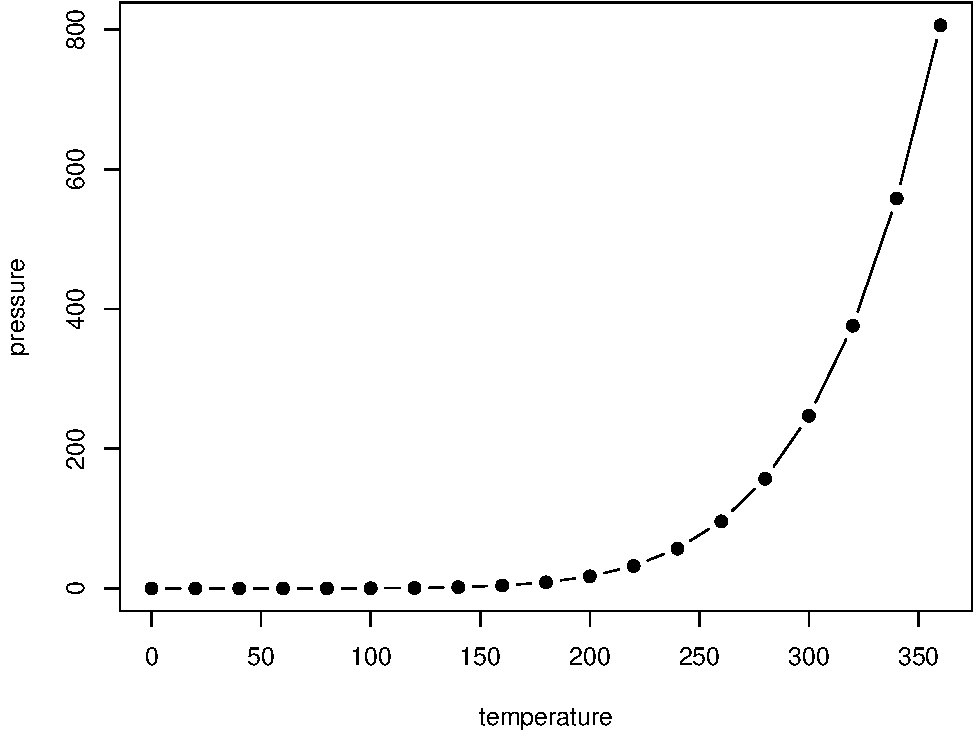
\includegraphics[width=0.8\linewidth]{_main_files/figure-latex/nice-fig-1} 

}

\caption{Here is a nice figure!}\label{fig:nice-fig}
\end{figure}

Reference a figure by its code chunk label with the \texttt{fig:} prefix, e.g., see Figure \ref{fig:nice-fig}. Similarly, you can reference tables generated from \texttt{knitr::kable()}, e.g., see Table \ref{tab:nice-tab}.

\begin{Shaded}
\begin{Highlighting}[]
\NormalTok{knitr}\SpecialCharTok{::}\FunctionTok{kable}\NormalTok{(}
  \FunctionTok{head}\NormalTok{(iris, }\DecValTok{20}\NormalTok{), }\AttributeTok{caption =} \StringTok{\textquotesingle{}Here is a nice table!\textquotesingle{}}\NormalTok{,}
  \AttributeTok{booktabs =} \ConstantTok{TRUE}
\NormalTok{)}
\end{Highlighting}
\end{Shaded}

\begin{table}

\caption{\label{tab:nice-tab}Here is a nice table!}
\centering
\begin{tabular}[t]{rrrrl}
\toprule
Sepal.Length & Sepal.Width & Petal.Length & Petal.Width & Species\\
\midrule
5.1 & 3.5 & 1.4 & 0.2 & setosa\\
4.9 & 3.0 & 1.4 & 0.2 & setosa\\
4.7 & 3.2 & 1.3 & 0.2 & setosa\\
4.6 & 3.1 & 1.5 & 0.2 & setosa\\
5.0 & 3.6 & 1.4 & 0.2 & setosa\\
\addlinespace
5.4 & 3.9 & 1.7 & 0.4 & setosa\\
4.6 & 3.4 & 1.4 & 0.3 & setosa\\
5.0 & 3.4 & 1.5 & 0.2 & setosa\\
4.4 & 2.9 & 1.4 & 0.2 & setosa\\
4.9 & 3.1 & 1.5 & 0.1 & setosa\\
\addlinespace
5.4 & 3.7 & 1.5 & 0.2 & setosa\\
4.8 & 3.4 & 1.6 & 0.2 & setosa\\
4.8 & 3.0 & 1.4 & 0.1 & setosa\\
4.3 & 3.0 & 1.1 & 0.1 & setosa\\
5.8 & 4.0 & 1.2 & 0.2 & setosa\\
\addlinespace
5.7 & 4.4 & 1.5 & 0.4 & setosa\\
5.4 & 3.9 & 1.3 & 0.4 & setosa\\
5.1 & 3.5 & 1.4 & 0.3 & setosa\\
5.7 & 3.8 & 1.7 & 0.3 & setosa\\
5.1 & 3.8 & 1.5 & 0.3 & setosa\\
\bottomrule
\end{tabular}
\end{table}

You can write citations, too. For example, we are using the \textbf{bookdown} package \citep{R-bookdown} in this sample book, which was built on top of R Markdown and \textbf{knitr} \citep{xie2015}.

\hypertarget{specification-and-standard-assumptions}{%
\chapter{Specification and standard assumptions}\label{specification-and-standard-assumptions}}

\hypertarget{specification}{%
\section{Specification}\label{specification}}

\begin{center}\rule{0.5\linewidth}{0.5pt}\end{center}

\begin{definition}
\protect\hypertarget{def:essai}{}\label{def:essai}A linear regression is a model defined through:
\[
y_i = \boldsymbol\beta'{\bf x}_{i} + \varepsilon_i,
\]
where \({\bf x}_{i}=[x_{i,1},\dots,x_{i,K}]'\) is a vector of dimension \(K \times 1\).
\end{definition}

\begin{center}\rule{0.5\linewidth}{0.5pt}\end{center}

For entity \(i\), the \(x_{i,k}\)'s, for \(k \in \{1,\dots,K\}\), are explanatory variables. If one wants to have an intercept in the specification, then set \(x_{i,1}=1\) for all \(i\), and \(\beta_1\) then corresponds to the intercept.

\begin{center}\rule{0.5\linewidth}{0.5pt}\end{center}

\begin{hypothesis}[Full rank]
\protect\hypertarget{hyp:fullrank}{}\label{hyp:fullrank}There is no exact linear relationship among the independent variables (the \(x_{i,k}\)s, for a given \(i \in \{1,\dots,n\}\)).
\end{hypothesis}

\begin{center}\rule{0.5\linewidth}{0.5pt}\end{center}

\begin{center}\rule{0.5\linewidth}{0.5pt}\end{center}

\begin{hypothesis}[Conditional mean-zero assumption]
\protect\hypertarget{hyp:exogeneity}{}\label{hyp:exogeneity}\begin{equation}
\mathbb{E}(\boldsymbol\varepsilon|\mathbf{X}) = 0.
\end{equation}
\end{hypothesis}

\begin{center}\rule{0.5\linewidth}{0.5pt}\end{center}

Note that, in Hypothesis \ref{hyp:exogeneity}, \(\boldsymbol\varepsilon\) is a \(n\)-dimensional vector (where \(n\) is the sample size), and \(\mathbf{X}\) is the matrix containing all explanatory variables, of dimension \(n \times K\).

\begin{center}\rule{0.5\linewidth}{0.5pt}\end{center}

\begin{proposition}
\protect\hypertarget{prp:implicationExog}{}\label{prp:implicationExog}

Under Hypothesis \ref{hyp:exogeneity}:

\begin{enumerate}
\def\labelenumi{\roman{enumi}.}
\item
  \(\mathbb{E}(\varepsilon_{i})=0\);
\item
  the \(x_{ij}\)s and the \(\varepsilon_{i}\)s are uncorrelated, i.e.~\(\forall i,\,j \quad \mathbb{C}orr(x_{ij},\varepsilon_{i})=0\).
\end{enumerate}

\end{proposition}

\begin{center}\rule{0.5\linewidth}{0.5pt}\end{center}

\begin{proof}

Let us prove (i) and (ii):

\begin{enumerate}
\def\labelenumi{\roman{enumi}.}
\tightlist
\item
  By the law of iterated expectations:
  \[
  \mathbb{E}(\boldsymbol\varepsilon)=\mathbb{E}(\mathbb{E}(\boldsymbol\varepsilon|\mathbf{X}))=\mathbb{E}(0)=0.
  \]
\item
  \(\mathbb{E}(x_{ij}\varepsilon_i)=\mathbb{E}(\mathbb{E}(x_{ij}\varepsilon_i|\mathbf{X}))=\mathbb{E}(x_{ij}\underbrace{\mathbb{E}(\varepsilon_i|\mathbf{X})}_{=0})=0\).\(\square\)
\end{enumerate}

\end{proof}

\begin{center}\rule{0.5\linewidth}{0.5pt}\end{center}

\begin{hypothesis}[Homoskedasticity]
\protect\hypertarget{hyp:homoskedasticity}{}\label{hyp:homoskedasticity}\[
\forall i, \quad \mathbb{V}ar(\varepsilon_i|\mathbf{X}) = \sigma^2.
\]
\end{hypothesis}

\begin{center}\rule{0.5\linewidth}{0.5pt}\end{center}

\begin{figure}

{\centering 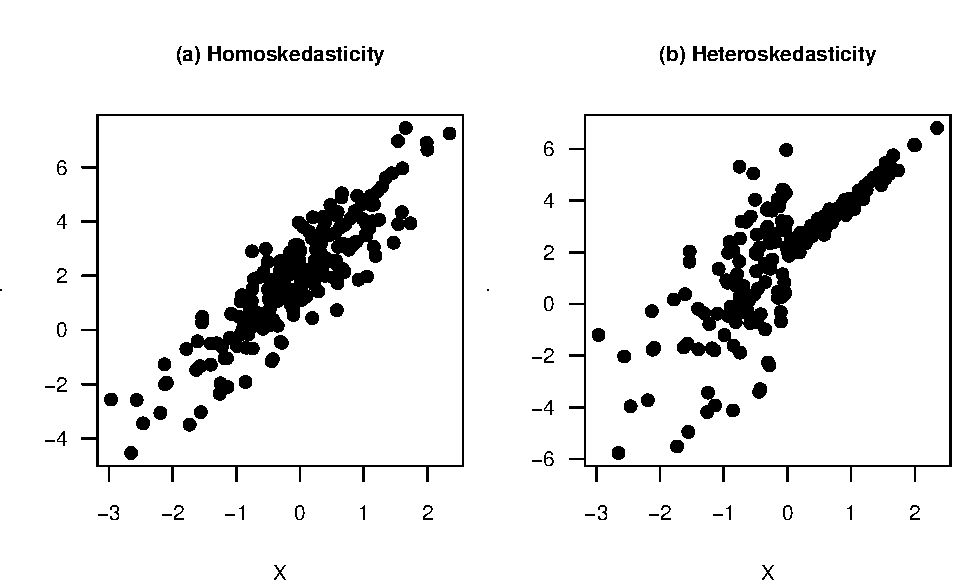
\includegraphics[width=0.9\linewidth]{_main_files/figure-latex/heteroskedasticity-1} 

}

\caption{This is the caption}\label{fig:heteroskedasticity}
\end{figure}

Panel (b) of Figure \ref{fig:heteroskedasticity} corresponds to a situation of heteroskedasticity. Let us be more specific. In the two plots, we have \(X_i \sim \mathcal{N}(0,1)\) and \(\varepsilon^*_i \sim \mathcal{N}(0,1)\). In Panel (a) (homoskedasticity): \(Y_i = 2 + 2X_i + \varepsilon^*_i\). In Panel (b) (heteroskedasticity): \(Y_i = 2 + 2X_i + \left(2\mathbb{1}_{\{X_i<0\}}+0.2\mathbb{1}_{\{X_i\ge0\}}\right)\varepsilon^*_i\).

\begin{Shaded}
\begin{Highlighting}[]
\CommentTok{\# load data into R}
\FunctionTok{data}\NormalTok{(Salaries, }\AttributeTok{package =} \StringTok{"carData"}\NormalTok{)}
\CommentTok{\# six first rows of the data}
\FunctionTok{head}\NormalTok{(Salaries)}
\end{Highlighting}
\end{Shaded}

\begin{verbatim}
##        rank discipline yrs.since.phd yrs.service  sex salary
## 1      Prof          B            19          18 Male 139750
## 2      Prof          B            20          16 Male 173200
## 3  AsstProf          B             4           3 Male  79750
## 4      Prof          B            45          39 Male 115000
## 5      Prof          B            40          41 Male 141500
## 6 AssocProf          B             6           6 Male  97000
\end{verbatim}

\begin{Shaded}
\begin{Highlighting}[]
\CommentTok{\# Regression:}
\NormalTok{eq }\OtherTok{\textless{}{-}} \FunctionTok{lm}\NormalTok{(salary}\SpecialCharTok{\textasciitilde{}}\NormalTok{.,}\AttributeTok{data=}\NormalTok{Salaries)}
\FunctionTok{summary}\NormalTok{(eq)}
\end{Highlighting}
\end{Shaded}

\begin{verbatim}
## 
## Call:
## lm(formula = salary ~ ., data = Salaries)
## 
## Residuals:
##    Min     1Q Median     3Q    Max 
## -65248 -13211  -1775  10384  99592 
## 
## Coefficients:
##               Estimate Std. Error t value Pr(>|t|)    
## (Intercept)    65955.2     4588.6  14.374  < 2e-16 ***
## rankAssocProf  12907.6     4145.3   3.114  0.00198 ** 
## rankProf       45066.0     4237.5  10.635  < 2e-16 ***
## disciplineB    14417.6     2342.9   6.154 1.88e-09 ***
## yrs.since.phd    535.1      241.0   2.220  0.02698 *  
## yrs.service     -489.5      211.9  -2.310  0.02143 *  
## sexMale         4783.5     3858.7   1.240  0.21584    
## ---
## Signif. codes:  0 '***' 0.001 '**' 0.01 '*' 0.05 '.' 0.1 ' ' 1
## 
## Residual standard error: 22540 on 390 degrees of freedom
## Multiple R-squared:  0.4547, Adjusted R-squared:  0.4463 
## F-statistic:  54.2 on 6 and 390 DF,  p-value: < 2.2e-16
\end{verbatim}

\begin{Shaded}
\begin{Highlighting}[]
\FunctionTok{par}\NormalTok{(}\AttributeTok{mfrow=}\FunctionTok{c}\NormalTok{(}\DecValTok{1}\NormalTok{,}\DecValTok{1}\NormalTok{))}
\FunctionTok{par}\NormalTok{(}\AttributeTok{plt=}\FunctionTok{c}\NormalTok{(.}\DecValTok{2}\NormalTok{,.}\DecValTok{95}\NormalTok{,.}\DecValTok{2}\NormalTok{,.}\DecValTok{95}\NormalTok{))}
\FunctionTok{plot}\NormalTok{(salary}\SpecialCharTok{/}\DecValTok{1000}\SpecialCharTok{\textasciitilde{}}\NormalTok{yrs.since.phd,}\AttributeTok{pch=}\DecValTok{19}\NormalTok{,}\AttributeTok{xlab=}\StringTok{"years since PhD"}\NormalTok{,}\AttributeTok{ylab=}\StringTok{"Salary"}\NormalTok{,}\AttributeTok{data=}\NormalTok{Salaries,}\AttributeTok{las=}\DecValTok{1}\NormalTok{)}
\FunctionTok{abline}\NormalTok{(}\FunctionTok{lm}\NormalTok{(salary}\SpecialCharTok{/}\DecValTok{1000}\SpecialCharTok{\textasciitilde{}}\NormalTok{yrs.since.phd,}\AttributeTok{data=}\NormalTok{Salaries),}\AttributeTok{col=}\StringTok{"red"}\NormalTok{,}\AttributeTok{lwd=}\DecValTok{2}\NormalTok{)}
\end{Highlighting}
\end{Shaded}

\begin{figure}

{\centering 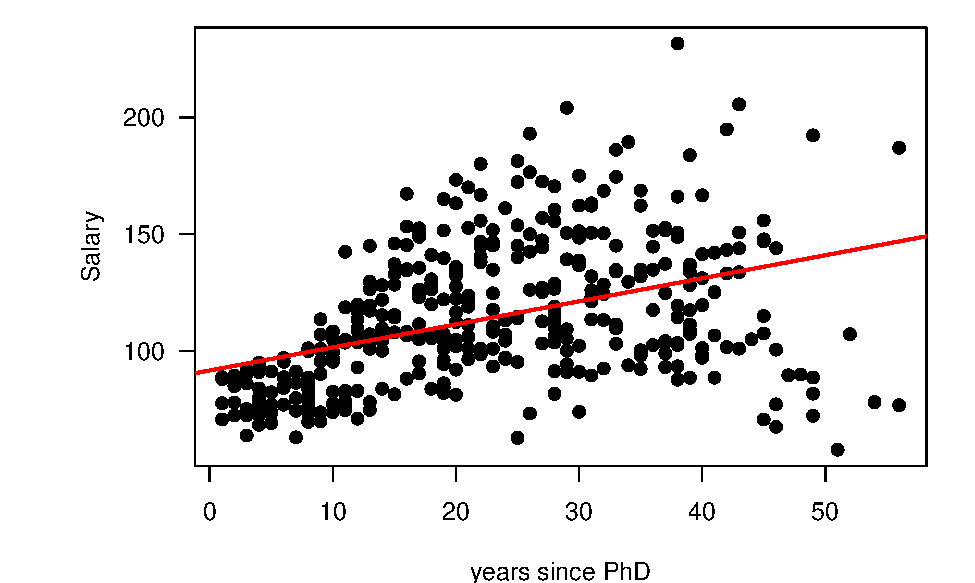
\includegraphics[width=0.9\linewidth]{_main_files/figure-latex/exmpSalarayPhD-1} 

}

\caption{Salary versus years after PhD}\label{fig:exmpSalarayPhD}
\end{figure}

\begin{center}\rule{0.5\linewidth}{0.5pt}\end{center}

\begin{hypothesis}[Uncorrelated residuals]
\protect\hypertarget{hyp:noncorrelResid}{}\label{hyp:noncorrelResid}\[
\forall i \ne j, \quad \mathbb{C}ov(\varepsilon_i,\varepsilon_j|\mathbf{X})=0.
\]
\end{hypothesis}

\begin{center}\rule{0.5\linewidth}{0.5pt}\end{center}

\begin{center}\rule{0.5\linewidth}{0.5pt}\end{center}

\begin{proposition}
\protect\hypertarget{prp:Sigma}{}\label{prp:Sigma}If \ref{hyp:homoskedasticity} and \ref{hyp:noncorrelResid} hold, then:
\[
\mathbb{V}ar(\boldsymbol\varepsilon|\mathbf{X})= \sigma^2 Id,
\]
where \(Id\) is the \(n \times n\) identity matrix.
\end{proposition}

\begin{center}\rule{0.5\linewidth}{0.5pt}\end{center}

\begin{center}\rule{0.5\linewidth}{0.5pt}\end{center}

\begin{hypothesis}[Normal distribution]
\protect\hypertarget{hyp:normality}{}\label{hyp:normality}\[
\forall i, \quad \varepsilon_i \sim \mathcal{N}(0,\sigma^2).
\]
\end{hypothesis}

\begin{center}\rule{0.5\linewidth}{0.5pt}\end{center}

\hypertarget{least-square-estimation}{%
\section{Least square estimation}\label{least-square-estimation}}

For a given vector of coefficients \(\mathbf{b}=[b_1,\dots,b_K]'\), the sum of square residuals is:
\[
f(\mathbf{b}) =\sum_{i=1}^n \left(y_i - \sum_{j=1}^K x_{i,j} b_j \right)^2 = \sum_{i=1}^n (y_i - \mathbf{x}_i' \mathbf{b})^2.
\]
Minimizing the sum of squared residuals amounts to minimizing:
\[
f(\mathbf{b}) = (\mathbf{y} - \mathbf{X}\mathbf{b})'(\mathbf{y} - \mathbf{X}\mathbf{b}).
\]

We have:
\[
\frac{\partial f}{\partial \mathbf{b}}(\mathbf{b}) = - 2 \mathbf{X}'\mathbf{y} + 2 \mathbf{X}'\mathbf{X}\mathbf{b}.
\]
Necessary first-order condition (FOC):
\begin{equation}
\mathbf{X}'\mathbf{X}\mathbf{b} = \mathbf{X}'\mathbf{y}.\label{eq:OLSFOC}
\end{equation}
Under Assumption \ref{hyp:fullrank}, \(\mathbf{X}'\mathbf{X}\) is invertible. Hence:
\[
\boxed{\mathbf{b} = (\mathbf{X}'\mathbf{X})^{-1} \mathbf{X}'\mathbf{y}.}
\]
Vector \(\mathbf{b}\) minimises the sum of squared residuals. (\(f\) is a non-negative quadratic function, it admits a minimum.)

The estimated residuals are:
\begin{equation}
\mathbf{e} = \mathbf{y} - \mathbf{X} (\mathbf{X}'\mathbf{X})^{-1} \mathbf{X}' \mathbf{y} = \mathbf{M} \mathbf{y}\label{eq:Mres}
\end{equation}
where \(\mathbf{M} := \mathbf{I} - \mathbf{X} (\mathbf{X}'\mathbf{X})^{-1} \mathbf{X}'\) is called the \textbf{residual maker} matrix. Let us further define a \textbf{projection matrix} by \(\mathbf{P}=\mathbf{X} (\mathbf{X}'\mathbf{X})^{-1} \mathbf{X}'\). These matrices \(\mathbf{M}\) and \(\mathbf{P}\) are such that:

\begin{itemize}
\tightlist
\item
  \(\mathbf{M} \mathbf{X} = \mathbf{0}\): if one regresses one of the explanatory variables on \(\mathbf{X}\), the residuals are null.
\item
  \(\mathbf{M}\mathbf{y}=\mathbf{M}\boldsymbol\varepsilon\) (because \(\mathbf{y} = \mathbf{X}\boldsymbol\beta + \boldsymbol\varepsilon\) and \(\mathbf{M} \mathbf{X} = \mathbf{0}\)).
\item
  The fitted values are:
  \begin{equation}
  \hat{\mathbf{y}}=\mathbf{X} (\mathbf{X}'\mathbf{X})^{-1} \mathbf{X}' \mathbf{y} = \mathbf{P} \mathbf{y},\label{eq:Proj}
  \end{equation}
  i.e., \(\hat{\mathbf{y}}\) is the projection of the vector \(\mathbf{y}\) onto the vectorial space spanned by the columns of \(\mathbf{X}\).
\item
  It can be shown that each column \(\tilde{\mathbf{x}}_k\) of \(\mathbf{X}\) is orthogonal to \(\mathbf{e}\). \(\Rightarrow\) If intercepts are included in the regression (\(x_{i,1} \equiv 1\)), the average of the residuals is null.
\end{itemize}

Here are some properties of \(\mathbf{M}\) and \(\mathbf{P}\):

\begin{itemize}
\tightlist
\item
  \(\mathbf{M}\) is symmetric (\(\mathbf{M} = \mathbf{M}'\)) and \textbf{idempotent} (\(\mathbf{M} = \mathbf{M}^2 = \mathbf{M}^k\) for \(k>0\)).
\item
  \(\mathbf{P}\) is symmetric and idempotent.
\item
  \(\mathbf{P}\mathbf{X} = \mathbf{X}\).
\item
  \(\mathbf{P} \mathbf{M} = \mathbf{M} \mathbf{P} = 0\).
\item
  \(\mathbf{y} = \mathbf{P}\mathbf{y} + \mathbf{M}\mathbf{y}\) (decomposition of \(\mathbf{y}\) into two orthogonal parts).
\end{itemize}

\begin{center}\rule{0.5\linewidth}{0.5pt}\end{center}

\begin{proposition}[Properties of the OLS estimator]
\protect\hypertarget{prp:propOLS}{}\label{prp:propOLS}

We have:

\begin{enumerate}
\def\labelenumi{\roman{enumi}.}
\item
  Under Assumptions \ref{hyp:fullrank} and \ref{hyp:exogeneity}, the OLS estimator is linear and unbiased.
\item
  Under Hypotheses \ref{hyp:fullrank} to \ref{hyp:noncorrelResid}, the conditional covariance matrix of \(\mathbf{b}\) is: \(\mathbb{V}ar(\mathbf{b}|\mathbf{X}) = \sigma^2 (\mathbf{X}'\mathbf{X})^{-1}\).
\end{enumerate}

\end{proposition}

\begin{center}\rule{0.5\linewidth}{0.5pt}\end{center}

\begin{proof}

Under Hypothesis \ref{hyp:fullrank}, \(\mathbf{X}'\mathbf{X}\) can be inverted. We have:
\[
\mathbf{b} = (\mathbf{X}'\mathbf{X})^{-1} \mathbf{X}'\mathbf{y} = \boldsymbol\beta + (\mathbf{X}'\mathbf{X})^{-1} \mathbf{X}' \mathbf{\varepsilon}.
\]

\begin{enumerate}
\def\labelenumi{\roman{enumi}.}
\tightlist
\item
  Let us consider the expectation of the last term, i.e.~\(\mathbb{E}((\mathbf{X}'\mathbf{X})^{-1} \mathbf{X}' \mathbf{\varepsilon})\). Using the law of iterated expectations, we obtain:
  \[
  \mathbb{E}((\mathbf{X}'\mathbf{X})^{-1} \mathbf{X}' \mathbf{\varepsilon}) = \mathbb{E}(\mathbb{E}[(\mathbf{X}'\mathbf{X})^{-1} \mathbf{X}' \mathbf{\varepsilon}|\mathbf{X}]) = \mathbb{E}((\mathbf{X}'\mathbf{X})^{-1} \mathbf{X}'\mathbb{E}[\mathbf{\varepsilon}|\mathbf{X}]).
  \]
  By Hypothesis \ref{hyp:exogeneity}, we have \(\mathbb{E}[\mathbf{\varepsilon}|\mathbf{X}]=0\). Hence \(\mathbb{E}((\mathbf{X}'\mathbf{X})^{-1} \mathbf{X}' \mathbf{\varepsilon}) =0\) and result (i) follows.
\item
  \(\mathbb{V}ar(\mathbf{b}|\mathbf{X}) = (\mathbf{X}'\mathbf{X})^{-1} \mathbf{X}' \mathbb{E}(\boldsymbol\varepsilon\boldsymbol\varepsilon'|\mathbf{X}) \mathbf{X} (\mathbf{X}'\mathbf{X})^{-1}\).
  By Prop. \ref{prp:Sigma}, if \ref{hyp:homoskedasticity} and \ref{hyp:noncorrelResid} hold, then we have \(\mathbb{E}(\boldsymbol\varepsilon\boldsymbol\varepsilon'|\mathbf{X})=\mathbb{V}ar(\boldsymbol\varepsilon|\mathbf{X})=\sigma^2 Id\). The result follows. \(\square\)
\end{enumerate}

\end{proof}

\hypertarget{bivariate-case}{%
\section{Bivariate case}\label{bivariate-case}}

Consider a bivariate situation, where we regress\(y_i\) on a constant and an explanatory variable \(w_i\). We have \(K=2\), and \(\mathbf{X}\) is a \(n \times 2\) matrix whose \(i^{th}\) row is \([x_{i,1},x_{i,2}]\), with \(x_{i,1}=1\) (to account for the intercept) and with \(w_i = x_{i,2}\) (say).

We have:
\begin{eqnarray*}
\mathbf{X}'\mathbf{X} &=& 
\left[\begin{array}{cc}
n & \sum_i w_i \\
\sum_i w_i & \sum_i w_i^2
\end{array}
\right],\\
(\mathbf{X}'\mathbf{X})^{-1} &=& 
\frac{1}{n\sum_i w_i^2-(\sum_i w_i)^2}
\left[\begin{array}{cc}
\sum_i w_i^2 & -\sum_i w_i \\
-\sum_i w_i & n
\end{array}
\right],\\
(\mathbf{X}'\mathbf{X})^{-1}\mathbf{X}'\mathbf{y} &=& 
\frac{1}{n\sum_i w_i^2-(\sum_i w_i)^2}
\left[\begin{array}{c}
\sum_i w_i^2\sum_i y_i -\sum_i w_i \sum_i w_iy_i \\
-\sum_i w_i \sum_i y_i + n \sum_i w_i y_i
\end{array}
\right]\\
&=& \frac{1}{\frac{1}{n}\sum_i(w_i - \bar{w})^2}
\left[\begin{array}{c}
\frac{\bar{y}}{n}\sum_i w_i^2 -\frac{\bar{w}}{n}\sum_i w_iy_i \\
\frac{1}{n}\sum_i (w_i-\bar{w})(y_i-\bar{y})
\end{array}
\right].
\end{eqnarray*}

It can be seen that the second element of \(\mathbf{b}=(\mathbf{X}'\mathbf{X})^{-1}\mathbf{X}'\mathbf{y}\) is:
\[
b_2 = \frac{\overline{\mathbb{C}ov(W,Y)}}{\overline{\mathbb{V}ar(W)}},
\]
where \(\overline{\mathbb{C}ov(W,Y)}\) and \(\overline{\mathbb{V}ar(W)}\) are sample estimates.

Since there is a constant in the regression, we have \(b_1 = \bar{y} - b_2 \bar{w}\).

\hypertarget{gauss-markow-theorem}{%
\section{Gauss Markow Theorem}\label{gauss-markow-theorem}}

\begin{center}\rule{0.5\linewidth}{0.5pt}\end{center}

\begin{theorem}[Gauss-Markov Theorem]
\protect\hypertarget{thm:GaussMarkov}{}\label{thm:GaussMarkov}Under Assumptions \ref{hyp:fullrank} to \ref{hyp:noncorrelResid}, for any vector \(w\), the minimum-variance linear unbiased estimator of \(w' \boldsymbol\beta\) is \(w' \mathbf{b}\), where \(\mathbf{b}\) is the least squares estimator. (BLUE: Best Linear Unbiased Estimator.)
\end{theorem}

\begin{center}\rule{0.5\linewidth}{0.5pt}\end{center}

\begin{proof}
Consider \(\mathbf{b}^* = C \mathbf{y}\), another linear unbiased estimator of \(\boldsymbol\beta\). Since it is unbiased, we must have \(\mathbb{E}(C\mathbf{y}|\mathbf{X}) = \mathbb{E}(C\mathbf{X}\boldsymbol\beta + C\boldsymbol\varepsilon|\mathbf{X}) = \boldsymbol\beta\). We have \(\mathbb{E}(C\boldsymbol\varepsilon|\mathbf{X})=C\mathbb{E}(\boldsymbol\varepsilon|\mathbf{X})=0\) (by \ref{hyp:exogeneity}).

Therefore \(\mathbf{b}^*\) is unbiased if \(\mathbb{E}(C\mathbf{X})\boldsymbol\beta=\boldsymbol\beta\). This has to be the case for any \(\boldsymbol\beta\), which implies that we must have \(C\mathbf{X}=\mathbf{I}\).\textbackslash{}

Let us compute \(\mathbb{V}ar(\mathbf{b^*}|\mathbf{X})\). For this, we introduce \(D = C - (\mathbf{X}'\mathbf{X})^{-1}\mathbf{X}'\), which is such that \(D\mathbf{y}=\mathbf{b}^*-\mathbf{b}\). The fact that \(C\mathbf{X}=\mathbf{I}\) implies that \(D\mathbf{X} = \mathbf{0}\).

We have \(\mathbb{V}ar(\mathbf{b^*}|\mathbf{X}) = \mathbb{V}ar(C \mathbf{y}|\mathbf{X}) =\mathbb{V}ar(C \boldsymbol\varepsilon|\mathbf{X}) = \sigma^2CC'\) (by Assumptions \ref{hyp:homoskedasticity} and \ref{hyp:noncorrelResid}, see Prop. \ref{prp:Sigma}). Using \(C=D+(\mathbf{X}'\mathbf{X})^{-1}\mathbf{X}'\) and exploiting the fact that \(D\mathbf{X} = \mathbf{0}\) leads to:
\[
\mathbb{V}ar(\mathbf{b^*}|\mathbf{X}) =\sigma^2\left[(D+(\mathbf{X}'\mathbf{X})^{-1}\mathbf{X}')(D+(\mathbf{X}'\mathbf{X})^{-1}\mathbf{X}')'\right] = \mathbb{V}ar(\mathbf{b}|\mathbf{X}) + \sigma^2 \mathbf{D}\mathbf{D}'.
\]
Therefore, we have \(\mathbb{V}ar(w'\mathbf{b^*}|\mathbf{X})=w'\mathbb{V}ar(\mathbf{b}|\mathbf{X})w + \sigma^2 w'\mathbf{D}\mathbf{D}'w\ge w'\mathbb{V}ar(\mathbf{b}|\mathbf{X})w=\mathbb{V}ar(w'\mathbf{b}|\mathbf{X})\). \(\square\)
\end{proof}

\hypertarget{frish-waugh}{%
\section{Frish-Waugh}\label{frish-waugh}}

Consider the linear least square regression of \(\mathbf{y}\) on \(\mathbf{X}\). We introduce the notations:

\begin{itemize}
\tightlist
\item
  \(\mathbf{b}^{\mathbf{y}/\mathbf{X}}\): OLS estimates of \(\boldsymbol\beta\),
\item
  \(\mathbf{M}^{\mathbf{X}}\): residual-maker matrix of any regression on \(\mathbf{X}\),
\item
  \(\mathbf{P}^{\mathbf{X}}\): projection matrix of any regression on \(\mathbf{X}\).
\end{itemize}

Consider the case where we have two sets of explanatory variables: \(\mathbf{X} = [\mathbf{X}_1,\mathbf{X}_2]\). With obvious notations: \(\mathbf{b}^{\mathbf{y}/\mathbf{X}}=[\mathbf{b}_1',\mathbf{b}_2']'\).

\begin{center}\rule{0.5\linewidth}{0.5pt}\end{center}

\begin{theorem}[Frisch-Waugh Theorem]
\protect\hypertarget{thm:FW}{}\label{thm:FW}We have:
\[
\mathbf{b}_2 = \mathbf{b}^{\mathbf{M^{\mathbf{X}_1}y}/\mathbf{M^{\mathbf{X}_1}\mathbf{X}_2}}.
\]
\end{theorem}

\begin{center}\rule{0.5\linewidth}{0.5pt}\end{center}

\begin{proof}
The minimization of the least squares leads to (these are first-order conditions, see Eq. \eqref{eq:OLSFOC}):
\[
\left[ \begin{array}{cc} \mathbf{X}_1'\mathbf{X}_1 & \mathbf{X}_1'\mathbf{X}_2 \\ \mathbf{X}_2'\mathbf{X}_1 & \mathbf{X}_2'\mathbf{X}_2\end{array}\right]
\left[ \begin{array}{c} \mathbf{b}_1 \\ \mathbf{b}_2\end{array}\right] =
\left[ \begin{array}{c} \mathbf{X}_1' \mathbf{y} \\ \mathbf{X}_2' \mathbf{y} \end{array}\right].
\]
Use the first-row block of equations to solve for \(\mathbf{b}_1\) first; it comes as a function of \(\mathbf{b}_2\). Then use the second set of equations to solve for \(\mathbf{b}_2\), which leads to:
\[
\mathbf{b}_2 = [\mathbf{X}_2'\mathbf{X}_2 - \mathbf{X}_2'\mathbf{X}_1(\mathbf{X}_1'\mathbf{X}_1)\mathbf{X}_1'\mathbf{X}_2]^{-1}\mathbf{X}_2'(Id - \mathbf{X}_1(\mathbf{X}_1'\mathbf{X}_1)\mathbf{X}_1')\mathbf{y}=[\mathbf{X}_2' \mathbf{M}^{\mathbf{X}_1}\mathbf{X}_2]^{-1}\mathbf{X}_2'\mathbf{M}^{\mathbf{X}_1}\mathbf{y}.
\]
Using the fact that \(\mathbf{M}^{\mathbf{X}_1}\) is idempotent and symmetric leads to the result.\qed
\end{proof}

This suggests a second way of estimating \(\mathbf{b}_2\):

\begin{enumerate}
\def\labelenumi{\arabic{enumi}.}
\tightlist
\item
  Regress \(Y\) on \(X_1\), regress \(X_2\) on \(X_1\).
\item
  Regress the former residuals on the latter.
\end{enumerate}

\begin{Shaded}
\begin{Highlighting}[]
\NormalTok{Data }\OtherTok{\textless{}{-}} \FunctionTok{read.csv}\NormalTok{(}\StringTok{"https://raw.githubusercontent.com/jrenne/Data4courses/master/parapluie/data4parapluie.csv"}\NormalTok{)}
\NormalTok{dummies }\OtherTok{\textless{}{-}} \FunctionTok{as.matrix}\NormalTok{(Data[,}\DecValTok{4}\SpecialCharTok{:}\DecValTok{14}\NormalTok{])}
\NormalTok{eq\_all }\OtherTok{\textless{}{-}} \FunctionTok{lm}\NormalTok{(parapluie}\SpecialCharTok{\textasciitilde{}}\NormalTok{precip}\SpecialCharTok{+}\NormalTok{dummies,}\AttributeTok{data=}\NormalTok{Data)}
\FunctionTok{summary}\NormalTok{(eq\_all)}\SpecialCharTok{$}\NormalTok{coefficients}
\end{Highlighting}
\end{Shaded}

\begin{verbatim}
##                Estimate Std. Error    t value     Pr(>|t|)
## (Intercept)  -2.9534478 3.40601605 -0.8671268 0.3893855798
## precip        0.1300055 0.03594492  3.6167985 0.0006192876
## dummiesX1    -8.5990682 3.30046623 -2.6054101 0.0115966151
## dummiesX2   -13.3290386 3.30657128 -4.0310755 0.0001613897
## dummiesX3    -7.9829582 3.25949898 -2.4491366 0.0173091333
## dummiesX4    -3.3923533 3.27605582 -1.0354992 0.3046614769
## dummiesX5    -3.7038158 3.25710094 -1.1371511 0.2600724511
## dummiesX6    -3.3606412 3.27334327 -1.0266694 0.3087670632
## dummiesX7    -7.3158812 3.28491529 -2.2271141 0.0297682836
## dummiesX8    -7.7172773 3.26128164 -2.3663327 0.0212677987
## dummiesX9    -4.6491997 3.26005024 -1.4261129 0.1591057652
## dummiesX10   -5.1091987 3.25143961 -1.5713651 0.1214457733
## dummiesX11    1.9807700 3.25942144  0.6077060 0.5457145714
\end{verbatim}

\begin{Shaded}
\begin{Highlighting}[]
\NormalTok{deseas\_parapluie }\OtherTok{\textless{}{-}} \FunctionTok{lm}\NormalTok{(parapluie}\SpecialCharTok{\textasciitilde{}}\NormalTok{dummies,}\AttributeTok{data=}\NormalTok{Data)}\SpecialCharTok{$}\NormalTok{residuals}
\NormalTok{deseas\_precip    }\OtherTok{\textless{}{-}} \FunctionTok{lm}\NormalTok{(precip}\SpecialCharTok{\textasciitilde{}}\NormalTok{dummies,}\AttributeTok{data=}\NormalTok{Data)}\SpecialCharTok{$}\NormalTok{residuals}
\NormalTok{eq\_frac }\OtherTok{\textless{}{-}} \FunctionTok{lm}\NormalTok{(deseas\_parapluie}\SpecialCharTok{\textasciitilde{}}\NormalTok{deseas\_precip)}
\FunctionTok{summary}\NormalTok{(eq\_frac)}\SpecialCharTok{$}\NormalTok{coefficients}
\end{Highlighting}
\end{Shaded}

\begin{verbatim}
##                    Estimate Std. Error       t value     Pr(>|t|)
## (Intercept)   -3.265931e-16 0.60898084 -5.362946e-16 1.0000000000
## deseas_precip  1.300055e-01 0.03300004  3.939557e+00 0.0001907741
\end{verbatim}

When \(b_2\) is scalar (and then \(\mathbf{X}_2\) is of dimension \(n \times 1\)), Theorem \ref{thm:FW} leads to:
\[
b_2 = \frac{\mathbf{X}_2'M^{\mathbf{X}_1}\mathbf{y}}{\mathbf{X}_2'M^{\mathbf{X}_1}\mathbf{X}_2} \quad \text{(partial regression coefficient)}.
\]

\hypertarget{goodness-of-fit}{%
\section{Goodness of fit}\label{goodness-of-fit}}

Define the total variation in \(y\) as the sum of squared deviations:
\[
TSS = \sum_{i=1}^{n} (y_i - \bar{y})^2.
\]
We have:
\[
\mathbf{y} = \mathbf{X}\mathbf{b} + \mathbf{e} = \hat{\mathbf{y}} + \mathbf{e}
\]
In the following, we assume that the regression includes a constant (i.e.~for all \(i\), \(x_{i,1}=1\)). Denote by \(\mathbf{M}^0\) the matrix that transforms observations into deviations from sample means. Using that \(\mathbf{M}^0 \mathbf{e} = \mathbf{e}\) and that \(\mathbf{X}' \mathbf{e}=0\), we have:
\begin{eqnarray*}
\underbrace{\mathbf{y}'\mathbf{M}^0\mathbf{y}}_{\mbox{Total sum of sq.}} &=& (\mathbf{X}\mathbf{b} + \mathbf{e})' \mathbf{M}^0 (\mathbf{X}\mathbf{b} + \mathbf{e})\\
&=& \underbrace{\mathbf{b}' \mathbf{X}' \mathbf{M}^0 \mathbf{X}\mathbf{b}}_{\mbox{"Explained" sum of sq.}} + \underbrace{\mathbf{e}'\mathbf{e}}_{\mbox{Sum of sq. residuals}}\\
TSS &=& Expl.SS + SSR.
\end{eqnarray*}

\begin{equation}
\boxed{\mbox{Coefficient of determination} = \frac{Expl.SS}{TSS} = 1 - \frac{SSR}{TSS} = 1 - \frac{\mathbf{e}'\mathbf{e}}{\mathbf{y}'\mathbf{M}^0\mathbf{y}}.}\label{eq:RR2}
\end{equation}

It can be shown {[}Greene, 2012, Section 3.5{]} that:
\[
\mbox{Coefficient of determination} = \frac{[\sum_{i=1}^n(y_i - \bar{y})(\hat{y_i} - \bar{y})]^2}{\sum_{i=1}^n(y_i - \bar{y})^2 \sum_{i=1}^n(\hat{y_i} - \bar{y})^2}.
\]
\(\Rightarrow\) \(R^2\) is the sample squared correlation between \(y\) and the (regression-implied) \(y\)'s predictions.

\begin{Shaded}
\begin{Highlighting}[]
\FunctionTok{par}\NormalTok{(}\AttributeTok{mfrow=}\FunctionTok{c}\NormalTok{(}\DecValTok{1}\NormalTok{,}\DecValTok{2}\NormalTok{))}
\FunctionTok{par}\NormalTok{(}\AttributeTok{plt=}\FunctionTok{c}\NormalTok{(.}\DecValTok{3}\NormalTok{,.}\DecValTok{95}\NormalTok{,.}\DecValTok{2}\NormalTok{,.}\DecValTok{85}\NormalTok{))}
\NormalTok{N }\OtherTok{\textless{}{-}} \DecValTok{100}
\NormalTok{eps }\OtherTok{\textless{}{-}} \FunctionTok{rnorm}\NormalTok{(N)}
\NormalTok{X }\OtherTok{\textless{}{-}} \FunctionTok{rnorm}\NormalTok{(N)}
\NormalTok{Y }\OtherTok{\textless{}{-}} \DecValTok{1} \SpecialCharTok{+}\NormalTok{ X }\SpecialCharTok{+}\NormalTok{ eps}
\FunctionTok{plot}\NormalTok{(X,Y,}\AttributeTok{pch=}\DecValTok{19}\NormalTok{,}\AttributeTok{main=}\StringTok{"(a) Low R2"}\NormalTok{)}
\NormalTok{Y }\OtherTok{\textless{}{-}} \DecValTok{1} \SpecialCharTok{+}\NormalTok{ X }\SpecialCharTok{+}\NormalTok{ .}\DecValTok{1}\SpecialCharTok{*}\NormalTok{eps}
\FunctionTok{plot}\NormalTok{(X,Y,}\AttributeTok{pch=}\DecValTok{19}\NormalTok{,}\AttributeTok{main=}\StringTok{"(b) High R2"}\NormalTok{)}
\end{Highlighting}
\end{Shaded}

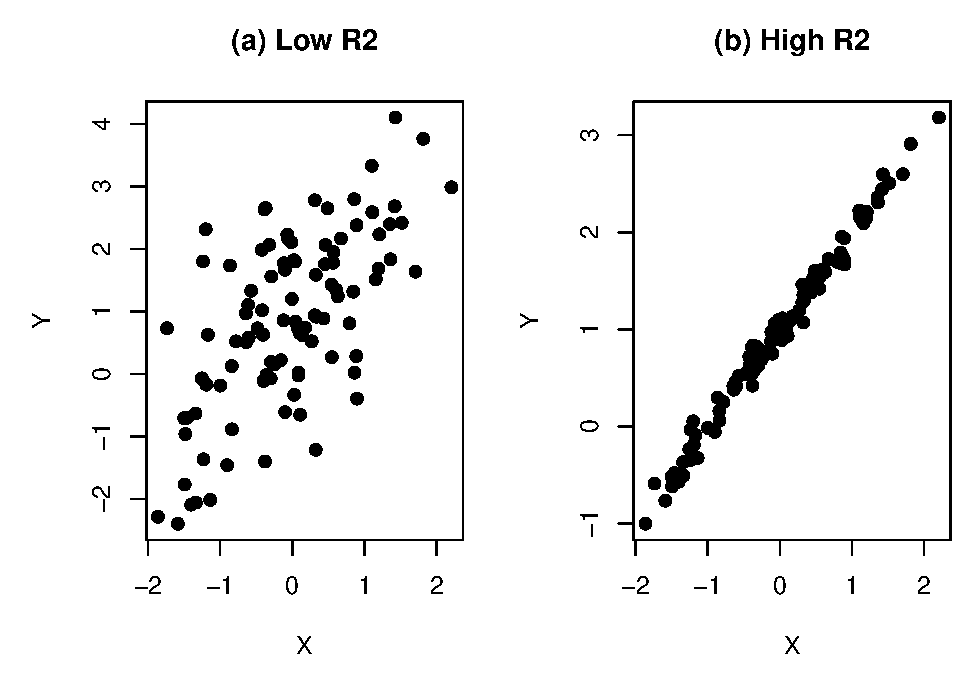
\includegraphics{_main_files/figure-latex/R2-1.pdf}

The \textbf{partial correlation} between \(y\) and \(z\), controlling for some variables \(\mathbf{X}\) is the sample correlation between \(y^*\) and \(z^*\), where the latter two variables are the residuals in regressions of \(y\) on \(\mathbf{X}\) and of \(z\) on \(\mathbf{X}\), respectively.

This correlation is denoted by \(r_{yz}^\mathbf{X}\). By definition, we have:
\begin{equation}
r_{yz}^\mathbf{X} = \frac{\mathbf{z^*}'\mathbf{y^*}}{\sqrt{(\mathbf{z^*}'\mathbf{z^*})(\mathbf{y^*}'\mathbf{y^*})}}.\label{eq:pc}
\end{equation}

\begin{center}\rule{0.5\linewidth}{0.5pt}\end{center}

\begin{proposition}[Change in SSR when a variable is added]
\protect\hypertarget{prp:chgeR2}{}\label{prp:chgeR2}We have:
\begin{equation}
\mathbf{u}'\mathbf{u} = \mathbf{e}'\mathbf{e} - c^2(\mathbf{z^*}'\mathbf{z^*}) \qquad (\le \mathbf{e}'\mathbf{e}) \label{eq:uu}
\end{equation}
where (i) \(\mathbf{u}\) and \(\mathbf{e}\) are the residuals in the regressions of \(\mathbf{y}\) on \([\mathbf{X},\mathbf{z}]\) and of \(\mathbf{y}\) on \(\mathbf{X}\), respectively, (ii) \(c\) is the regression coefficient on \(\mathbf{z}\) in the former regression and where \(\mathbf{z}^*\) are the residuals in the regression of \(\mathbf{z}\) on \(\mathbf{X}\).
\end{proposition}

\begin{center}\rule{0.5\linewidth}{0.5pt}\end{center}

\begin{proof}
The OLS estimates \([\mathbf{d}',\mathbf{c}]'\) in the regression of \(\mathbf{y}\) on \([\mathbf{X},\mathbf{z}]\) satisfies (first-order cond., Eq. \eqref{eq:OLSFOC})
\[
\left[ \begin{array}{cc} \mathbf{X}'\mathbf{X} & \mathbf{X}'\mathbf{z} \\ \mathbf{z}'\mathbf{X} & \mathbf{z}'\mathbf{z}\end{array}\right]
\left[ \begin{array}{c} \mathbf{d} \\ \mathbf{c}\end{array}\right] =
\left[ \begin{array}{c} \mathbf{X}' \mathbf{y} \\ \mathbf{z}' \mathbf{y} \end{array}\right].
\]
Hence, in particular \(\mathbf{d} = \mathbf{b} - (\mathbf{X}'\mathbf{X})^{-1}\mathbf{X}'\mathbf{z}\mathbf{c}\), where \(\mathbf{b}\) is the OLS of \(\mathbf{y}\) on \(\mathbf{X}\). Substituting in \(\mathbf{u} = \mathbf{y} - \mathbf{X}\mathbf{d} - \mathbf{z}c\), we get \(\mathbf{u} = \mathbf{e} - \mathbf{z}^*c\). We therefore have:
\begin{equation}
\mathbf{u}'\mathbf{u} = (\mathbf{e} - \mathbf{z}^*c)(\mathbf{e} - \mathbf{z}^*c)= \mathbf{e}'\mathbf{e} + c^2(\mathbf{z^*}'\mathbf{z^*}) - 2 c\mathbf{z^*}'\mathbf{e}.\label{eq:uuu}
\end{equation}
Now \(\mathbf{z^*}'\mathbf{e} = \mathbf{z^*}'(\mathbf{y} - \mathbf{X}\mathbf{b}) = \mathbf{z^*}'\mathbf{y}\) because \(\mathbf{z}^*\) are the residuals in an OLS regression on \(\mathbf{X}\). Since \(c = (\mathbf{z^*}'\mathbf{z^*})^{-1}\mathbf{z^*}'\mathbf{y^*}\) (by an application of Theorem \ref{thm:FW}), we have \((\mathbf{z^*}'\mathbf{z^*})c = \mathbf{z^*}'\mathbf{y^*}\) and, therefore, \(\mathbf{z^*}'\mathbf{e} = (\mathbf{z^*}'\mathbf{z^*})c\). Inserting this in Eq. \eqref{eq:uuu} leads to the results. \(\square\)
\end{proof}

\begin{center}\rule{0.5\linewidth}{0.5pt}\end{center}

\begin{proposition}[Change in the coefficient of determination when a variable is added]
\protect\hypertarget{prp:chgeInR2}{}\label{prp:chgeInR2}Denoting by \(R_W^2\) the coefficient of determination in the regression of \(\mathbf{y}\) on some variable \(\mathbf{W}\), we have:
\[
R_{\mathbf{X},\mathbf{z}}^2 = R_{\mathbf{X}}^2 + (1-R_{\mathbf{X}}^2)(r_{yz}^\mathbf{X})^2,
\]
where \(r_{yz}^\mathbf{X}\) is the coefficient of partial correlation.
\end{proposition}

\begin{proof}
Let's use the same notations as in Prop. @ref\{prp:chgeR2\}. Theorem \ref{thm:FW} implies that \(c = (\mathbf{z^*}'\mathbf{z^*})^{-1}\mathbf{z^*}'\mathbf{y^*}\). Using this in Eq. \eqref{eq:uu} gives \(\mathbf{u}'\mathbf{u} = \mathbf{e}'\mathbf{e} - (\mathbf{z^*}'\mathbf{y^*})^2/(\mathbf{z^*}'\mathbf{z^*})\). Using the definition of the partial correlation (Eq. \eqref{eq:pc}), we get \(\mathbf{u}'\mathbf{u} = \mathbf{e}'\mathbf{e}\left(1 - (r_{yz}^\mathbf{X})^2\right)\). The results is obtained by dividing both sides of the previous equation by \(\mathbf{y}'\mathbf{M}_0\mathbf{y}\). \(\square\)
\end{proof}

The previous theorem shows that we necessarily increase the \(R^2\) if we add variables, \textbf{even if they are irrelevant}.

The \textbf{adjusted \(R^2\)}, denoted by \(\bar{R}^2\), is a fit measure that penalizes large numbers of regressors:
\begin{equation*}
\boxed{\bar{R}^2 = 1 - \frac{\mathbf{e}'\mathbf{e}/(n-K)}{\mathbf{y}'\mathbf{M}^0\mathbf{y}/(n-1)} = 1 - \frac{n-1}{n-K}(1-R^2).}
\end{equation*}

\hypertarget{inference-and-prediction}{%
\section{Inference and Prediction}\label{inference-and-prediction}}

Under the normality assumption (Assumption \ref{hyp:normality}), we know the distribution of \(\mathbf{b}\) (conditional on \(\mathbf{X}\)). Indeed, \((\mathbf{b}|\mathbf{X}) \equiv (\mathbf{X}'\mathbf{X})^{-1} \mathbf{X}'\mathbf{y}\) is multivariate Gaussian:
\begin{equation}
\mathbf{b}|\mathbf{X} \sim \mathcal{N}(\beta,\sigma^2(\mathbf{X}'\mathbf{X})^{-1}).\label{eq:distriBcondi}
\end{equation}

Problem: In practice, we do not know \(\sigma^2\) (\textbf{population parameter}).

\begin{center}\rule{0.5\linewidth}{0.5pt}\end{center}

\begin{proposition}
\protect\hypertarget{prp:expects2}{}\label{prp:expects2}Under \ref{hyp:fullrank} to \ref{hyp:noncorrelResid}, an unbiased estimate of \(\sigma^2\) is given by:
\begin{equation}
s^2 = \frac{\mathbf{e}'\mathbf{e}}{n-K}.\label{eq:s2}
\end{equation}
(It is sometimes denoted by \(\sigma^2_{OLS}\).)
\end{proposition}

\begin{center}\rule{0.5\linewidth}{0.5pt}\end{center}

\begin{proof}
\(\mathbb{E}(\mathbf{e}'\mathbf{e}|\mathbf{X})=\mathbb{E}(\boldsymbol{\varepsilon}'\mathbf{M}\boldsymbol{\varepsilon}|\mathbf{X})=\mathbb{E}(\mbox{Tr}(\boldsymbol{\varepsilon}'\mathbf{M}\boldsymbol{\varepsilon})|\mathbf{X})) =\mbox{Tr}(\mathbf{M}\mathbb{E}(\boldsymbol{\varepsilon}\boldsymbol{\varepsilon}'|\mathbf{X}))=\sigma^2 \mbox{Tr}(\mathbf{M})\). (Note that we have \(\mathbb{E}(\boldsymbol{\varepsilon}\boldsymbol{\varepsilon}'|\mathbf{X})=\sigma^2Id\) by Assumptions \ref{hyp:homoskedasticity} and \ref{hyp:noncorrelResid}, see Prop. \ref{prp:Sigma}.) Finally: \(\mbox{Tr}(\mathbf{M})=n-\mbox{Tr}(\mathbf{X}(\mathbf{X}'\mathbf{X})^{-1}\mathbf{X}')=n-\mbox{Tr}((\mathbf{X}'\mathbf{X})^{-1}\mathbf{X}'\mathbf{X})=n-\mbox{Tr}(Id_{K\times K})\). \(\square\)
\end{proof}

Two results will prove important to perform hypothesis testing:

\begin{enumerate}
\def\labelenumi{\roman{enumi}.}
\tightlist
\item
  We know the distribution of \(s^2\) (Prop. \ref{prp:s2distri}).
\item
  \(s^2\) and \(\mathbf{b}\) are independent random variables (Prop. \ref{prp:indeps2b}).
\end{enumerate}

\begin{center}\rule{0.5\linewidth}{0.5pt}\end{center}

\begin{proposition}
\protect\hypertarget{prp:s2distri}{}\label{prp:s2distri}Under \ref{hyp:fullrank} to \ref{hyp:normality}, we have: \(\dfrac{s^2}{\sigma^2} | \mathbf{X} \sim \chi^2(n-K)/(n-K)\).
\end{proposition}

\begin{center}\rule{0.5\linewidth}{0.5pt}\end{center}

\begin{proof}
We have \(\mathbf{e}'\mathbf{e}=\boldsymbol\varepsilon'\mathbf{M}\boldsymbol\varepsilon\). \(\mathbf{M}\) is an idempotent symmetric matrix. Therefore it can be decomposed as \(PDP'\) where \(D\) is a diagonal matrix and \(P\) is an orthogonal matrix. As a result \(\mathbf{e}'\mathbf{e} = (P'\boldsymbol\varepsilon)'D(P'\boldsymbol\varepsilon)\), i.e.~\(\mathbf{e}'\mathbf{e}\) is a weighted sum of independent squared Gaussian variables (the entries of \(P'\boldsymbol\varepsilon\) are independent because they are Gaussian -- under \ref{hyp:normality} -- and uncorrelated). The variance of each of these i.i.d. Gaussian variable is \(\sigma^2\). Because \(\mathbf{M}\) is an idempotent symmetric matrix, its eigenvalues are either 0 or 1, and its rank equals its trace. Further, its trace is equal to \(n-K\) (see proof of Eq. \eqref{eq:s2}). Therefore \(D\) has \(n-K\) entries equal to 1 and \(K\) equal to 0.Hence, \(\mathbf{e}'\mathbf{e} = (P'\boldsymbol\varepsilon)'D(P'\boldsymbol\varepsilon)\) is a sum of \(n-K\) squared independent Gaussian variables of variance \(\sigma^2\). Therefore \(\frac{\mathbf{e}'\mathbf{e}}{\sigma^2} = (n-K)\frac{s^2}{\sigma^2}\) is a sum of \(n-k\) squared i.i.d. standard normal variables. \(\square\)
\end{proof}

\begin{center}\rule{0.5\linewidth}{0.5pt}\end{center}

\begin{proposition}
\protect\hypertarget{prp:indeps2b}{}\label{prp:indeps2b}Under Hypotheses \ref{hyp:fullrank} to \ref{hyp:normality}, \(\mathbf{b}\) and \(s^2\) are independent.
\end{proposition}

\begin{center}\rule{0.5\linewidth}{0.5pt}\end{center}

\begin{proof}
We have \(\mathbf{b}=\boldsymbol\beta + [\mathbf{X}'{\mathbf{X}}]^{-1}\mathbf{X}\boldsymbol\varepsilon\) and \(s^2 = \boldsymbol\varepsilon' \mathbf{M} \boldsymbol\varepsilon/(n-K)\). Hence \(\mathbf{b}\) is an affine combination of \(\boldsymbol\varepsilon\) and \(s^2\) is a quadratic combination of the same Gaussian shocks. One can write \(s^2\) as \(s^2 = (\mathbf{M}\boldsymbol\varepsilon)' \mathbf{M} \boldsymbol\varepsilon/(n-K)\) and \(\mathbf{b}\) as \(\boldsymbol\beta + \mathbf{T}\boldsymbol\varepsilon\). Since \(\mathbf{T}\mathbf{M}=0\), \(\mathbf{T}\boldsymbol\varepsilon\) and \(\mathbf{M}\boldsymbol\varepsilon\) are independent (because two uncorrelated Gaussian variables are independent), therefore \(\mathbf{b}\) and \(s^2\), which are functions of respective independent variables, are independent. \(\square\)
\end{proof}

Under Hypotheses \ref{hyp:fullrank} to \ref{hyp:normality}, let us consider \(b_k\), the \(k^{th}\) entry of \(\mathbf{b}\):
\[
b_k | \mathbf{X} \sim \mathcal{N}(\beta_k,\sigma^2 v_k),
\]
where \(v_k\) is the k\(^{th}\) component of the diagonal of \((\mathbf{X}'\mathbf{X})^{-1}\).

Besides, we have (Prop. \ref{prp:s2distri}):
\[
\frac{(n-K)s^2}{\sigma^2} | \mathbf{X} \sim \chi ^2 (n-K).
\]

As a result (using Props. \ref{prp:s2distri} and \ref{prp:indeps2b}), we have:
\begin{equation}
\boxed{t_k = \frac{\frac{b_k - \beta_k}{\sqrt{\sigma^2 v_k}}}{\sqrt{\frac{(n-K)s^2}{\sigma^2(n-K)}}} = \frac{b_k - \beta_k}{\sqrt{s^2v_k}} \sim t(n-K),}\label{eq:resultstudentt}
\end{equation}
where \(t(n-K)\) denotes a \(t\) distribution with \(n-K\) degrees of freedom.

Remark: \(\frac{b_k - \beta_k}{\sqrt{\sigma^2 v_k}} | \mathbf{X} \sim \mathcal{N}(0,1)\) and \(\frac{(n-K)s^2}{\sigma^2} | \mathbf{X} \sim \chi ^2 (n-K)\). These two distributions do not depend on \(\mathbf{X}\) \(\Rightarrow\) the \emph{marginal distribution} of \(t_k\) is also \(t\).

Note that \(s^2 v_k\) is not exactly the conditional variance of \(b_k\): The variance of \(b_k\) conditional on \(\mathbf{X}\) is \(\sigma^2 v_k\). However \(s^2 v_k\) is an unbiased estimate of \(\sigma^2 v_k\) (by Prop. \ref{prp:expects2}).

The previous result (Eq. \eqref{eq:resultstudentt}) can be extended to any linear combinations of elements of \(\mathbf{b}\) (Eq. \eqref{eq:resultstudentt} is for its \(k^{th}\) component only).

Let us consider \(\boldsymbol\alpha'\mathbf{b}\), the OLS estimate of \(\boldsymbol\alpha'\boldsymbol\beta\). From Eq. \eqref{eq:distriBcondi}, we have:
\[
\boldsymbol\alpha'\mathbf{b} | \mathbf{X} \sim \mathcal{N}(\boldsymbol\alpha'\boldsymbol\beta,\sigma^2 \boldsymbol\alpha'(\mathbf{X}'\mathbf{X})^{-1}\boldsymbol\alpha).
\]
Therefore:
\[
\frac{\boldsymbol\alpha'\mathbf{b} - \boldsymbol\alpha'\boldsymbol\beta}{\sqrt{\sigma^2 \boldsymbol\alpha'(\mathbf{X}'\mathbf{X})^{-1}\boldsymbol\alpha}} | \mathbf{X} \sim \mathcal{N}(0,1).
\]
Using the same approach as the one used to derive Eq. \eqref{eq:resultstudentt}, one can show that Props. \ref{prp:s2distri} and \ref{prp:indeps2b} imply that:
\begin{equation}
\boxed{\frac{\boldsymbol\alpha'\mathbf{b} - \boldsymbol\alpha'\boldsymbol\beta}{\sqrt{s^2\boldsymbol\alpha'(\mathbf{X}'\mathbf{X})^{-1}\boldsymbol\alpha}} \sim t(n-K).}\label{eq:resultstudentt2}
\end{equation}

\begin{Shaded}
\begin{Highlighting}[]
\FunctionTok{par}\NormalTok{(}\AttributeTok{plt=}\FunctionTok{c}\NormalTok{(.}\DecValTok{2}\NormalTok{,.}\DecValTok{95}\NormalTok{,.}\DecValTok{2}\NormalTok{,.}\DecValTok{95}\NormalTok{))}
\NormalTok{xx }\OtherTok{\textless{}{-}} \FunctionTok{seq}\NormalTok{(}\SpecialCharTok{{-}}\FloatTok{3.5}\NormalTok{,}\FloatTok{3.5}\NormalTok{,}\AttributeTok{by=}\NormalTok{.}\DecValTok{01}\NormalTok{)}
\FunctionTok{plot}\NormalTok{(xx,}\FunctionTok{dnorm}\NormalTok{(xx),}\AttributeTok{xlab=}\StringTok{"X"}\NormalTok{,}\AttributeTok{ylab=}\StringTok{""}\NormalTok{,}\AttributeTok{type=}\StringTok{"l"}\NormalTok{,}\AttributeTok{lwd=}\DecValTok{2}\NormalTok{)}
\FunctionTok{lines}\NormalTok{(xx,}\FunctionTok{dt}\NormalTok{(xx,}\AttributeTok{df=}\DecValTok{3}\NormalTok{),}\AttributeTok{col=}\StringTok{"red"}\NormalTok{,}\AttributeTok{lwd=}\DecValTok{2}\NormalTok{)}
\FunctionTok{lines}\NormalTok{(xx,}\FunctionTok{dt}\NormalTok{(xx,}\AttributeTok{df=}\DecValTok{7}\NormalTok{),}\AttributeTok{col=}\StringTok{"red"}\NormalTok{,}\AttributeTok{lwd=}\DecValTok{2}\NormalTok{,}\AttributeTok{lty=}\DecValTok{2}\NormalTok{)}
\FunctionTok{lines}\NormalTok{(xx,}\FunctionTok{dt}\NormalTok{(xx,}\AttributeTok{df=}\DecValTok{20}\NormalTok{),}\AttributeTok{col=}\StringTok{"blue"}\NormalTok{,}\AttributeTok{lwd=}\DecValTok{3}\NormalTok{,}\AttributeTok{lty=}\DecValTok{3}\NormalTok{)}
\FunctionTok{legend}\NormalTok{(}\StringTok{"topright"}\NormalTok{,}
       \FunctionTok{c}\NormalTok{(}\StringTok{"N(0,1)"}\NormalTok{,}\StringTok{"t(3)"}\NormalTok{,}\StringTok{"t(7)"}\NormalTok{,}\StringTok{"t(20)"}\NormalTok{),}
       \AttributeTok{lty=}\FunctionTok{c}\NormalTok{(}\DecValTok{1}\NormalTok{,}\DecValTok{1}\NormalTok{,}\DecValTok{2}\NormalTok{,}\DecValTok{3}\NormalTok{), }\CommentTok{\# gives the legend appropriate symbols (lines)       }
       \AttributeTok{lwd=}\FunctionTok{c}\NormalTok{(}\DecValTok{2}\NormalTok{,}\DecValTok{2}\NormalTok{,}\DecValTok{2}\NormalTok{,}\DecValTok{3}\NormalTok{), }\CommentTok{\# line width}
       \AttributeTok{col=}\FunctionTok{c}\NormalTok{(}\StringTok{"black"}\NormalTok{,}\StringTok{"red"}\NormalTok{,}\StringTok{"red"}\NormalTok{,}\StringTok{"blue"}\NormalTok{))}
\end{Highlighting}
\end{Shaded}

\begin{figure}
\centering
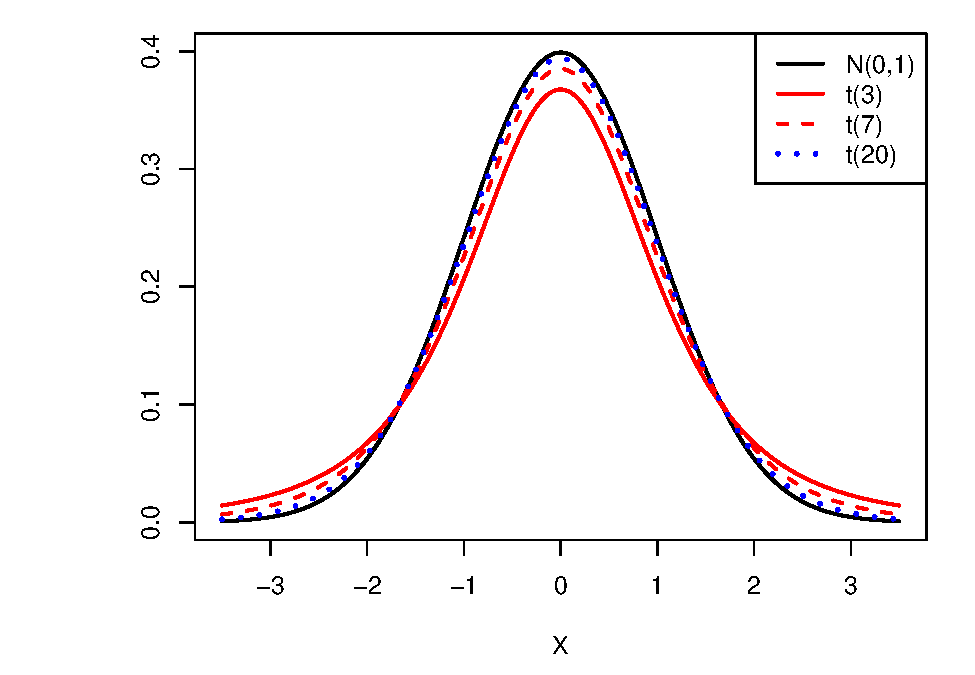
\includegraphics{_main_files/figure-latex/chartStudent-1.pdf}
\caption{\label{fig:chartStudent}The chart shows that the higher the degree of freedom, the closer the distribution of \(t( u)\) gets to the normal distribution.}
\end{figure}

\hypertarget{confidence-interval-of-beta_k}{%
\section{\texorpdfstring{Confidence interval of \(\beta_k\)}{Confidence interval of \textbackslash beta\_k}}\label{confidence-interval-of-beta_k}}

Assume we want to compute a (symmetrical) confidence interval \([I_{d,1-\alpha},I_{u,1-\alpha}]\) that is such that \(\mathbb{P}(\beta_k \in [I_{d,1-\alpha},I_{u,1-\alpha}])=1-\alpha\). In particular, we want to have: \(\mathbb{P}(\beta_k < I_{d,1-\alpha})=\frac{\alpha}{2}\).

For this purpose, we make use of \(t_k = \frac{b_k - \beta_k}{\sqrt{s^2v_k}} \sim t(n-K)\) (Eq. \eqref{eq:resultstudentt}).

We have:
\[
\mathbb{P}(\beta_k < I_{d,1-\alpha})=\frac{\alpha}{2} \Leftrightarrow
\]
\begin{eqnarray*}
\mathbb{P}\left(\frac{b_k - \beta_k}{\sqrt{s^2v_k}} > \frac{b_k - I_{d,1-\alpha}}{\sqrt{s^2v_k}}\right)=\frac{\alpha}{2} \Leftrightarrow \mathbb{P}\left(t_k > \frac{b_k - I_{d,1-\alpha}}{\sqrt{s^2v_k}}\right)=\frac{\alpha}{2} \Leftrightarrow&&\\
1 - \mathbb{P}\left(t_k \le \frac{b_k - I_{d,1-\alpha}}{\sqrt{s^2v_k}}\right)=\frac{\alpha}{2} \Leftrightarrow \frac{b_k - I_{d,1-\alpha}}{\sqrt{s^2v_k}} = \Phi^{-1}_{t(n-K)}\left(1-\frac{\alpha}{2}\right),&&
\end{eqnarray*}
where \(\Phi_{t(n-K)}(\alpha)\) is the c.d.f. of the \(t(n-K)\) distribution (Table @ref\{tab:Studenttable\}).

Doing the same for \(I_{u,1-\alpha}\), we obtain:
\begin{eqnarray*}
&&[I_{d,1-\alpha},I_{u,1-\alpha}] =\\
&&\left[b_k - \Phi^{-1}_{t(n-K)}\left(1-\frac{\alpha}{2}\right)\sqrt{s^2v_k},b_k + \Phi^{-1}_{t(n-K)}\left(1-\frac{\alpha}{2}\right)\sqrt{s^2v_k}\right].
\end{eqnarray*}

\hypertarget{example}{%
\subsection{Example}\label{example}}

The following example is based on the \href{https://hrs.isr.umich.edu/about}{HRS dataset (Health and Retirement Study)}. We only consider only a subset of this large dataset, focusing on a few variables, and for year 2018 (wave 14). This \href{https://raw.githubusercontent.com/jrenne/Data4courses/master/HRS_RAND/reduced_version/prepare_small_HRS.R}{R script} builds the reduced dataset.

\begin{Shaded}
\begin{Highlighting}[]
\NormalTok{reducedHRS }\OtherTok{\textless{}{-}} \FunctionTok{read.csv}\NormalTok{(}\StringTok{"https://raw.githubusercontent.com/jrenne/Data4courses/master/HRS\_RAND/reduced\_version/reducedHRS.csv"}\NormalTok{)}
\NormalTok{eq }\OtherTok{\textless{}{-}} \FunctionTok{lm}\NormalTok{(riearn}\SpecialCharTok{\textasciitilde{}}\NormalTok{raedyrs}\SpecialCharTok{+}\NormalTok{ragey\_b}\SpecialCharTok{+}\FunctionTok{I}\NormalTok{(ragey\_b}\SpecialCharTok{\^{}}\DecValTok{2}\NormalTok{)}\SpecialCharTok{+}\NormalTok{rfemale,}\AttributeTok{data=}\NormalTok{reducedHRS)}
\FunctionTok{print}\NormalTok{(}\FunctionTok{summary}\NormalTok{(eq))}
\end{Highlighting}
\end{Shaded}

\begin{verbatim}
## 
## Call:
## lm(formula = riearn ~ raedyrs + ragey_b + I(ragey_b^2) + rfemale, 
##     data = reducedHRS)
## 
## Residuals:
##    Min     1Q Median     3Q    Max 
## -82512 -29447  -8144  18083 394724 
## 
## Coefficients:
##                Estimate Std. Error t value Pr(>|t|)    
## (Intercept)  -1.336e+05  3.245e+04  -4.116 3.92e-05 ***
## raedyrs       5.216e+03  2.384e+02  21.876  < 2e-16 ***
## ragey_b       4.758e+03  1.086e+03   4.382 1.20e-05 ***
## I(ragey_b^2) -4.441e+01  9.097e+00  -4.882 1.09e-06 ***
## rfemale      -1.499e+04  1.498e+03 -10.007  < 2e-16 ***
## ---
## Signif. codes:  0 '***' 0.001 '**' 0.01 '*' 0.05 '.' 0.1 ' ' 1
## 
## Residual standard error: 50130 on 4540 degrees of freedom
## Multiple R-squared:  0.1173, Adjusted R-squared:  0.1165 
## F-statistic: 150.8 on 4 and 4540 DF,  p-value: < 2.2e-16
\end{verbatim}

The last two columns give the test statistic and p-values associated to the test whose null hypothesis is:
\[
H_0: \beta_k=0.
\]
The \textbf{t-statistics}, that is \(b_k/\sqrt{s^2 v_k}\), is the test statistic of the test. Under \(H_0\), the t-statistic is \(t(n-K)\) (see Eq. \eqref{eq:resultstudentt}). Hence, the \textbf{critical region} for the test of size \(\alpha\) is:
\[
\left]-\infty,-\Phi^{-1}_{t(n-K)}\left(1-\frac{\alpha}{2}\right)\right] \cup \left[\Phi^{-1}_{t(n-K)}\left(1-\frac{\alpha}{2}\right),+\infty\right[.
\]
The \textbf{p-value} is defined as the probability that \(|Z| > |t|\), where \(t\) is the (computed) t statistics and where \(Z \sim t(n-K)\). That is, the p-value is given by \(2(1 - \Phi_{t(n-K)}(|t_k|))\).

See \href{https://jrenne.shinyapps.io/tests/}{this webpage} for details regarding the link between critical regions, p-value, and test outcomes.

\hypertarget{set-of-linear-restrictions}{%
\section{Set of linear restrictions}\label{set-of-linear-restrictions}}

We consider the following model:
\[
\mathbf{y} = \mathbf{X}\boldsymbol\beta + \boldsymbol\varepsilon, \quad \varepsilon \sim i.i.d. \mathcal{N}(0,\sigma^2).
\]
and we want to test for the \emph{joint} validity of a set of restrictions involving the components of \(\boldsymbol\beta\) in a linear way.

Set of linear restrictions:
\begin{equation}\label{eq:restrictions}
\begin{array}{ccc}
r_{1,1} \beta_1 + \dots + r_{1,K} \beta_K &=& q_1\\
\vdots && \vdots\\
r_{J,1} \beta_1 + \dots + r_{J,K} \beta_K &=& q_J,
\end{array}
\end{equation}
that can be written in matrix form:
\begin{equation}
\mathbf{R}\boldsymbol\beta = \mathbf{q}.
\end{equation}

Defin the \textbf{Discrepancy vector} \(\mathbf{m} = \mathbf{R}\mathbf{b} - \mathbf{q}\). Under the null hypothesis:
\begin{eqnarray*}
\mathbb{E}(\mathbf{m}|\mathbf{X}) &=& \mathbf{R}\boldsymbol\beta - \mathbf{q} = 0 \quad \mbox{and} \\
\mathbb{V}ar(\mathbf{m}|\mathbf{X}) &=& \mathbf{R} \mathbb{V}ar(\mathbf{b}|\mathbf{X}) \mathbf{R}'.
\end{eqnarray*}
Under Hypotheses \ref{hyp:fullrank} to \ref{hyp:noncorrelResid}, \(\mathbb{V}ar(\mathbf{m}|\mathbf{X}) = \sigma^2 \mathbf{R} (\mathbf{X}'\mathbf{X})^{-1} \mathbf{R}'\) (see Prop. \ref{prp:propOLS}).

Consider the test:
\begin{equation}
\boxed{H_0: \mathbf{R}\boldsymbol\beta - \mathbf{q} = 0 \mbox{ against } H_1: \mathbf{R}\boldsymbol\beta - \mathbf{q} \ne 0.}\label{eq:H0Ftest}
\end{equation}

We could perform a \textbf{Wald test}. Under \ref{hyp:fullrank} to \ref{hyp:normality} --we need the normality assumption-- and under \(H_0\), it can be shown that we have:
\begin{equation}
W = \mathbf{m}'\mathbb{V}ar(\mathbf{m}|\mathbf{X})^{-1}\mathbf{m} \sim \chi^2(J). \label{eq:W1}
\end{equation}
However, \(\sigma^2\) is unknown. Hence we cannot compute \(W\).

We can however approximate it be replacing \(\sigma^2\) by \(s^2\). The distribution of this new statistic is not \(\chi^2(J)\) any more;
it is an \textbf{\(\mathcal{F}\) distribution}, and the test is called \textbf{\(F\) test}.

\begin{center}\rule{0.5\linewidth}{0.5pt}\end{center}

\begin{proposition}
\protect\hypertarget{prp:Ftest1}{}\label{prp:Ftest1}Under Hypotheses \ref{hyp:fullrank} to \ref{hyp:normality} and if Eq. \eqref{eq:H0Ftest} holds, we have:
\begin{equation}
F = \frac{W}{J}\frac{\sigma^2}{s^2} = \frac{\mathbf{m}'(\mathbf{R}(\mathbf{X}'\mathbf{X})^{-1}\mathbf{R}')^{-1}\mathbf{m}}{s^2J} \sim \mathcal{F}(J,n-K),\label{eq:defFstatistics}
\end{equation}
where \(\mathcal{F}\) is the distribution of the F-statistic.
\end{proposition}

\begin{center}\rule{0.5\linewidth}{0.5pt}\end{center}

\begin{proof}
According to Eq. \eqref{eq:W1}, \(W/J \sim \chi^2(J)/J\). Moreover, the denominator (\(s^2/\sigma^2\)) is \(\sim \chi^2(n-K)\). Therefore, \(F\) is the ratio of a r.v. distributed as \(\chi^2(J)/J\) and another distributed as \(\chi^2(n-K)/(n-K)\). It remains to verify that these r.v. are independent.

Under \(H_0\), we have \(\mathbf{m} = \mathbf{R}(\mathbf{b}-\boldsymbol\beta) = \mathbf{R}(\mathbf{X}'\mathbf{X})^{-1}\mathbf{X}'\boldsymbol\varepsilon\).
Therefore \(\mathbf{m}'(\mathbf{R}(\mathbf{X}'\mathbf{X})^{-1}\mathbf{R}')^{-1}\mathbf{m}\) is of the form \(\boldsymbol\varepsilon'\mathbf{T}\boldsymbol\varepsilon\) with \(\mathbf{T}=\mathbf{D}'\mathbf{C}\mathbf{D}\) where \(\mathbf{D}=\mathbf{R}(\mathbf{X}'\mathbf{X})^{-1}\mathbf{X}'\) and \(\mathbf{C}=(\mathbf{R}(\mathbf{X}'\mathbf{X})^{-1}\mathbf{R}')^{-1}\). Under Hypotheses \ref{hyp:fullrank} to \ref{hyp:noncorrelResid}, the covariance between \(\mathbf{T}\boldsymbol\varepsilon\) and \(\mathbf{M}\boldsymbol\varepsilon\) is \(\sigma^2\mathbf{T}\mathbf{M} = \mathbf{0}\). Therefore, under \ref{hyp:normality}, these variables are Gaussian variables with 0 covariance. Hence they are independent. \(\square\)
\end{proof}

Remark: For large \(n-K\), the \(\mathcal{F}_{J,n-K}\) distribution converges to \(\mathcal{F}_{J,\infty}=\chi^2(J)/J\).

\begin{center}\rule{0.5\linewidth}{0.5pt}\end{center}

\begin{proposition}
\protect\hypertarget{prp:Ftest}{}\label{prp:Ftest}The F-statistic defined by Eq. \eqref{eq:defFstatistics} is also equal to:
\begin{equation}
F = \frac{(R^2-R_*^2)/J}{(1-R^2)/(n-K)} =  \frac{(SSR_{restr}-SSR_{unrestr})/J}{SSR_{unrestr}/(n-K)},\label{eq:defFstatistics2}
\end{equation}
where \(R_*^2\) is the coef. of determination (Eq. \ref(eq:RR2)) of the ``restricted regression'\,' \emph{(SSR: sum of squared residuals.)}
\end{proposition}

\begin{center}\rule{0.5\linewidth}{0.5pt}\end{center}

\begin{proof}
Let's denote by \(\mathbf{e}_*=\mathbf{y}-\mathbf{X}\mathbf{b}_*\) the vector of residuals associated to the \emph{restricted regression} (i.e.~\(\mathbf{R}\mathbf{b}_*=\mathbf{q}\)).
We have \(\mathbf{e}_*=\mathbf{e} - \mathbf{X}(\mathbf{b}_*-\mathbf{b})\). Using \(\mathbf{e}'\mathbf{X}=0\), we get \(\mathbf{e}_*'\mathbf{e}_*=\mathbf{e}'\mathbf{e} + (\mathbf{b}_*-\mathbf{b})'\mathbf{X}'\mathbf{X}(\mathbf{b}_*-\mathbf{b}) \ge \mathbf{e}'\mathbf{e}\).

By Prop. @ref(prp:constrained\_LS), we know that \(\mathbf{b}_*-\mathbf{b}=-(\mathbf{X}'\mathbf{X})^{-1} \mathbf{R}'\{\mathbf{R}(\mathbf{X}'\mathbf{X})^{-1}\mathbf{R}'\}^{-1}(\mathbf{R}\mathbf{b} - \mathbf{q})\). Therefore:
\[
\mathbf{e}_*'\mathbf{e}_* - \mathbf{e}'\mathbf{e} = (\mathbf{R}\mathbf{b} - \mathbf{q})'[\mathbf{R}(\mathbf{X}'\mathbf{X})^{-1}\mathbf{R}']^{-1}(\mathbf{R}\mathbf{b} - \mathbf{q}).
\]
This implies that the F statistic defined in Prop. \ref{prp:Ftest1} is also equal to:
\[
\frac{(\mathbf{e}_*'\mathbf{e}_* - \mathbf{e}'\mathbf{e})/J}{\mathbf{e}'\mathbf{e}/(n-K)}. \square
\]
\end{proof}

The null hypothesis \(H_0\) (Eq. \eqref{eq:H0Ftest}) of the F-test is rejected if \(F\) --defined by Eq. \eqref{eq:defFstatistics} or \eqref{eq:defFstatistics2}-- is higher than \(\mathcal{F}_{1-\alpha}(J,n-K)\). (Hence, this test is a one-sided test.)

\hypertarget{common-pitfalls}{%
\section{Common pitfalls}\label{common-pitfalls}}

\hypertarget{multicollinearity}{%
\subsection{Multicollinearity}\label{multicollinearity}}

Consider the model: \(y_i = \beta_1 x_{i,1} + \beta_2 x_{i,2} + \varepsilon_i\), where all variables are zero-mean and \(\mathbb{V}ar(\varepsilon_i)=\sigma^2\). We have
\[
\mathbf{X}'\mathbf{X} = \left[ \begin{array}{cc}
\sum_i x_{i,1}^2 & \sum_i x_{i,1} x_{i,2} \\
\sum_i x_{i,1} x_{i,2} & \sum_i x_{i,2}^2
\end{array}\right],
\]
therefore:
\begin{eqnarray*}
(\mathbf{X}'\mathbf{X})^{-1} &=& \frac{1}{\sum_i x_{i,1}^2\sum_i x_{i,2}^2 - (\sum_i x_{i,1} x_{i,2})^2} \left[ \begin{array}{cc}
\sum_i x_{i,2}^2 & -\sum_i x_{i,1} x_{i,2} \\
-\sum_i x_{i,1} x_{i,2} & \sum_i x_{i,1}^2
\end{array}\right].
\end{eqnarray*}
The inverse of the upper-left parameter of \((\mathbf{X}'\mathbf{X})^{-1}\) is:
\begin{equation}
\sum_i x_{i,1}^2 - \frac{(\sum_i x_{i,1} x_{i,2})^2}{\sum_i x_{i,2}^2} = \sum_i x_{i,1}^2(1 - correl_{1,2}^2),\label{eq:multicollin}
\end{equation}
where \(correl_{1,2}\) is the sample correlation between \(\mathbf{x}_{1}\) and \(\mathbf{x}_{2}\).

Hence, the closer to one \(correl_{1,2}\), the higher the variance of \(b_1\) (recall that the variance of \(b_1\) is the upper-left component of \(\sigma^2(\mathbf{X}'\mathbf{X})^{-1}\)).

\hypertarget{omitted-variables}{%
\subsection{Omitted variables}\label{omitted-variables}}

Consider the following model, called ``True model'\,':
\[
\mathbf{y} = \underbrace{\mathbf{X}_1}_{n \times K_1}\underbrace{\boldsymbol\beta_1}_{K_1 \times 1} + \underbrace{\mathbf{X}_2}_{n\times K_2}\underbrace{\boldsymbol\beta_2}_{K_2 \times 1} + \boldsymbol\varepsilon
\]
Then, if one computes \(\mathbf{b}_1\) by regressing \(\mathbf{y}\) on \(\mathbf{X}_1\) only, we get:
\[
\mathbf{b}_1 = (\mathbf{X}_1'\mathbf{X}_1)^{-1}\mathbf{X}_1'\mathbf{y} = \boldsymbol\beta_1 + (\mathbf{X}_1'\mathbf{X}_1)^{-1}\mathbf{X}_1'\mathbf{X}_2\boldsymbol\beta_2 + 
(\mathbf{X}_1'\mathbf{X}_1)^{-1}\mathbf{X}_1'\boldsymbol\varepsilon.
\]

Hence, we obtain the omitted-variable formula:
\[
\boxed{\mathbb{E}(\mathbf{b}_1|\mathbf{X}) = \boldsymbol\beta_1 + \underbrace{(\mathbf{X}_1'\mathbf{X}_1)^{-1}(\mathbf{X}_1'\mathbf{X}_2)}_{K_1 \times K_2}\boldsymbol\beta_2}
\]
(each column of \((\mathbf{X}_1'\mathbf{X}_1)^{-1}(\mathbf{X}_1'\mathbf{X}_2)\) are the OLS regressors obtained when regressing the columns of \(\mathbf{X}_2\) on \(\mathbf{X}_1\)).

\begin{example}
\protect\hypertarget{exm:wageeduc}{}\label{exm:wageeduc}Consider the ``true model'\,':
\begin{equation}
wage_i = \beta_0 +\beta_1 edu_i + \beta_2 ability_i + \varepsilon_i, \quad \varepsilon_i \sim i.i.d.\,\mathcal{N}(0,\sigma_\varepsilon^2)
\end{equation}
Further, we assume that the \(edu\) variable is correlated to the \(ability\). Specifically:
\[
edu_i = \alpha_0 +\alpha_1 ability_i + \eta_i, \quad \eta_i \sim i.i.d.\,\mathcal{N}(0,\sigma_\eta^2).
\]
Assume we mistakingly run the regression omitting the \(ability\) variable:
\begin{equation}
wage_i = \gamma_0 +\gamma_1 edu_i + \xi_i.
\end{equation}
It can be seen that \(\xi_i = \varepsilon_i - (\beta_2/\alpha_1) \eta_i \sim i.i.d.\,\mathcal{N}(0,\sigma_\varepsilon^2+(\beta_2/\alpha_1)^2\sigma_\eta^2)\) and that the population regression coefficient is \(\gamma_1 = \beta_1 + \beta_2/\alpha_1 \ne \beta_1\).
\end{example}

\begin{example}
\protect\hypertarget{exm:CASchools}{}\label{exm:CASchools}

Let us use the \href{https://rdrr.io/cran/AER/man/CASchools.html}{California Test Score dataset} (in the package \texttt{AER}). Assume we want to measure the effect of the students-to-teacher ratio (`\texttt{str}) on student test scores (\texttt{testscr}). The folowing regressions show that the effect is lower when controls are added.

\begin{Shaded}
\begin{Highlighting}[]
\FunctionTok{library}\NormalTok{(AER); }\FunctionTok{data}\NormalTok{(}\StringTok{"CASchools"}\NormalTok{)}
\NormalTok{CASchools}\SpecialCharTok{$}\NormalTok{str }\OtherTok{\textless{}{-}}\NormalTok{ CASchools}\SpecialCharTok{$}\NormalTok{students}\SpecialCharTok{/}\NormalTok{CASchools}\SpecialCharTok{$}\NormalTok{teachers}
\NormalTok{CASchools}\SpecialCharTok{$}\NormalTok{testscr }\OtherTok{\textless{}{-}}\NormalTok{ .}\DecValTok{5} \SpecialCharTok{*}\NormalTok{ (CASchools}\SpecialCharTok{$}\NormalTok{math }\SpecialCharTok{+}\NormalTok{ CASchools}\SpecialCharTok{$}\NormalTok{read)}
\NormalTok{eq }\OtherTok{\textless{}{-}} \FunctionTok{lm}\NormalTok{(testscr}\SpecialCharTok{\textasciitilde{}}\NormalTok{str,}\AttributeTok{data=}\NormalTok{CASchools)}
\FunctionTok{summary}\NormalTok{(eq)}\SpecialCharTok{$}\NormalTok{coefficients}
\end{Highlighting}
\end{Shaded}

\begin{verbatim}
##               Estimate Std. Error   t value      Pr(>|t|)
## (Intercept) 698.932949  9.4674911 73.824516 6.569846e-242
## str          -2.279808  0.4798255 -4.751327  2.783308e-06
\end{verbatim}

\begin{Shaded}
\begin{Highlighting}[]
\NormalTok{eq }\OtherTok{\textless{}{-}} \FunctionTok{lm}\NormalTok{(testscr}\SpecialCharTok{\textasciitilde{}}\NormalTok{str}\SpecialCharTok{+}\NormalTok{lunch,}\AttributeTok{data=}\NormalTok{CASchools)}
\FunctionTok{summary}\NormalTok{(eq)}\SpecialCharTok{$}\NormalTok{coefficients}
\end{Highlighting}
\end{Shaded}

\begin{verbatim}
##                Estimate Std. Error    t value      Pr(>|t|)
## (Intercept) 702.9113020 4.70024626 149.547760  0.000000e+00
## str          -1.1172255 0.24035528  -4.648225  4.498554e-06
## lunch        -0.5997501 0.01676439 -35.775242 3.709097e-129
\end{verbatim}

\begin{Shaded}
\begin{Highlighting}[]
\NormalTok{eq }\OtherTok{\textless{}{-}} \FunctionTok{lm}\NormalTok{(testscr}\SpecialCharTok{\textasciitilde{}}\NormalTok{str}\SpecialCharTok{+}\NormalTok{lunch}\SpecialCharTok{+}\NormalTok{english,}\AttributeTok{data=}\NormalTok{CASchools)}
\FunctionTok{summary}\NormalTok{(eq)}\SpecialCharTok{$}\NormalTok{coefficients}
\end{Highlighting}
\end{Shaded}

\begin{verbatim}
##                Estimate Std. Error    t value     Pr(>|t|)
## (Intercept) 700.1499572 4.68568672 149.423126 0.000000e+00
## str          -0.9983090 0.23875428  -4.181324 3.535873e-05
## lunch        -0.5473454 0.02159885 -25.341418 2.303048e-86
## english      -0.1215735 0.03231728  -3.761872 1.928369e-04
\end{verbatim}

\end{example}

\hypertarget{irrelevant-variable}{%
\subsection{Irrelevant variable}\label{irrelevant-variable}}

Consider the \emph{True model}:
\[
\mathbf{y} = \mathbf{X}_1\boldsymbol\beta_1 + \boldsymbol\varepsilon,
\]
while the \emph{Estimated model} is:
\[
\mathbf{y} = \mathbf{X}_1\boldsymbol\beta_1 + \mathbf{X}_2\boldsymbol\beta_2 + \boldsymbol\varepsilon
\]

The estimates are unbiased. However, adding irrelevant explanatory variables increases the variance of the estimate of \(\boldsymbol\beta_1\) (compared to the case where one uses the correct explanatory variables). This is the case unless the correlation between \(\mathbf{X}_1\) and \(\mathbf{X}_2\) is null, see Eq. \eqref{eq:multicollin}.

In other words, the estimator is \emph{inefficient}, i.e., there exists an alternative consistent estimator whose variance is lower. The inefficiency problem can have serious consequences when testing hypotheses of type \(H_0: \beta_1 = 0\) due to the loss of power, so we might infer that they are no relevant variables when they truly are (Type-II error; False Negative).

\hypertarget{large-sample-properties}{%
\section{Large Sample Properties}\label{large-sample-properties}}

Even if we relax the normality assumption (Hypothesis \ref{hyp:normality}), we can approximate the finite-sample behavior of the estimators by using \emph{large-sample} or \emph{asymptotic properties}.

To begin with, we proceed under Hypothesis \ref{hyp:fullrank} to \ref{hyp:noncorrelResid}. (We will see later how to deal with --partial-- relaxations of Hypothesis \ref{hyp:homoskedasticity} and \ref{hyp:noncorrelResid}.)

Under regularity assumptions, under \ref{hyp:fullrank} to \ref{hyp:noncorrelResid}, even if the residuals are not normally-distributed, the least square estimators can be \emph{asymptotically normal} and inference can be performed as in small samples when \ref{hyp:fullrank} to \ref{hyp:normality} hold. This derives from Prop. \ref{prp:asymptOLS} (below). The F-test (Prop. \ref(prp:Ftest)) and the t-test can then be performed.

\begin{center}\rule{0.5\linewidth}{0.5pt}\end{center}

\begin{proposition}
\protect\hypertarget{prp:asymptOLS}{}\label{prp:asymptOLS}Under Assumptions \ref{hyp:fullrank} to \ref{hyp:noncorrelResid}, and assuming further that:
\begin{equation}
Q = \mbox{plim}_{n \rightarrow \infty} \frac{\mathbf{X}'\mathbf{X}}{n},\label{eq:Qasympt}
\end{equation}
and that the \((\mathbf{x}_i,\varepsilon_i)\)s are independent (across entities \(i\)), we have:
\begin{equation}
\sqrt{n}(\mathbf{b} - \boldsymbol\beta)\overset{d} {\rightarrow} \mathcal{N}\left(0,\sigma^2Q^{-1}\right).\label{eq:convgceOLS}
\end{equation}
\end{proposition}

\begin{center}\rule{0.5\linewidth}{0.5pt}\end{center}

\begin{proof}
Since \(\mathbf{b} = \boldsymbol\beta + \left( \frac{\mathbf{X}'\mathbf{X}}{n}\right)^{-1}\left(\frac{\mathbf{X}'\boldsymbol\varepsilon}{n}\right)\), we have: \(\sqrt{n}(\mathbf{b} - \boldsymbol\beta) = \left( \frac{\mathbf{X}'\mathbf{X}}{n}\right)^{-1} \left(\frac{1}{\sqrt{n}}\right)\mathbf{X}'\boldsymbol\varepsilon\). Since \(f:A \rightarrow A^{-1}\) is a continuous function (for \(A \ne \mathbf{0}\)), \(\mbox{plim}_{n \rightarrow \infty} \left(\frac{\mathbf{X}'\mathbf{X}}{n}\right)^{-1} = \mathbf{Q}^{-1}\). Let us denote by \(V_i\) the vector \(\mathbf{x}_i \varepsilon_i\). Because the \((\mathbf{x}_i,\varepsilon_i)\)s are independent, the \(V_i\)s are independent as well. Their covariance matrix is \(\sigma^2\mathbb{E}(\mathbf{x}_i \mathbf{x}_i')=\sigma^2Q\). Applying the multivariate central limit theorem on the \(V_i\)s gives \(\sqrt{n}\left(\frac{1}{n}\sum_{i=1}^n \mathbf{x}_i \varepsilon_i\right) = \left(\frac{1}{\sqrt{n}}\right)\mathbf{X}'\boldsymbol\varepsilon \overset{d}{\rightarrow} \mathcal{N}(0,\sigma^2Q)\). An application of Slutsky's theorem then leads to the results. \(\square\)
\end{proof}

In practice, \(\sigma^2\) is estimated with \(\frac{\mathbf{e}'\mathbf{e}}{n-K}\) (Eq. \eqref{eq:s2}) and \(\mathbf{Q}^{-1}\) with \(\left(\frac{\mathbf{X}'\mathbf{X}}{n}\right)^{-1}\).

Eqs. \eqref{eq:Qasympt} and \eqref{eq:convgceOLS} respectively correspond to convergences in probability and in distribution.

\hypertarget{instrumental-variables}{%
\section{Instrumental Variables}\label{instrumental-variables}}

Here, we want to relax Hypothesis \ref{hyp:exogeneity} --conditional mean zero assumption, implying in particular that \(\mathbf{x}_i\) and \(\varepsilon_i\) are uncorrelated.

We consider the following model:
\begin{equation}
y_i = \mathbf{x_i}'\boldsymbol\beta + \varepsilon_i, \quad \mbox{where } \mathbb{E}(\varepsilon_i)=0  \mbox{ and } \mathbf{x_i}\not\perp \varepsilon_i.\label{eq:modelIV}
\end{equation}

\begin{center}\rule{0.5\linewidth}{0.5pt}\end{center}

\begin{definition}
\protect\hypertarget{def:instruments}{}\label{def:instruments}

The \(L\)-dimensional random variable \(\mathbf{z}_i\) is a \textbf{valid set of instruments} if:

\begin{enumerate}
\def\labelenumi{\alph{enumi}.}
\tightlist
\item
  \(\mathbf{z}_i\) is correlated to \(\mathbf{x}_i\);
\item
  we have \(\mathbb{E}(\boldsymbol\varepsilon|\mathbf{Z})=0\) and
\item
  the orthogonal projections of the \(\mathbf{x}_i\)s on the \(\mathbf{z}_i\)s are not multicollinear.
\end{enumerate}

\end{definition}

\begin{center}\rule{0.5\linewidth}{0.5pt}\end{center}

Example. Let us make the assumption \(\mathbf{x}_i\not\perp \varepsilon_i\) (in \eqref{eq:modelIV}) more precise:
\begin{equation}
\mathbb{E}(\varepsilon_i)=0 \quad \mbox{and} \quad \mathbb{E}(\varepsilon_i \mathbf{x_i})=\boldsymbol\gamma.\label{eq:exmIV}
\end{equation}
By the law of large numbers, \(\mbox{plim}_{n \rightarrow \infty} \mathbf{X}'\boldsymbol\varepsilon / n = \boldsymbol\gamma\). If \(\mathbf{Q}_{xx} := \mbox{plim } \mathbf{X}'\mathbf{X}/n\), the OLS estimator is not consistent because
\[
\mathbf{b} = \boldsymbol\beta + (\mathbf{X}'\mathbf{X})^{-1}\mathbf{X}'\boldsymbol\varepsilon \overset{p}{\rightarrow} \boldsymbol\beta + \mathbf{Q}_{xx}^{-1}\boldsymbol\gamma \ne \boldsymbol\beta.
\]

If \(\mathbf{z}_i\) is a valid set of instruments, we have:
\[
\mbox{plim}\left( \frac{\mathbf{Z}'\mathbf{y}}{n} \right) =\mbox{plim}\left( \frac{\mathbf{Z}'(\mathbf{X}\boldsymbol\beta + \boldsymbol\varepsilon)}{n} \right) = \mbox{plim}\left( \frac{\mathbf{Z}'\mathbf{X}}{n} \right)\boldsymbol\beta
\]
Indeed, by the law of large numbers, \(\frac{\mathbf{Z}'\boldsymbol\varepsilon}{n} \overset{p}{\rightarrow}\mathbb{E}(\mathbf{z}_i\varepsilon_i)=0\).

If \(L = K\), the matrix \(\frac{\mathbf{Z}'\mathbf{X}}{n}\) is of dimension \(K \times K\) and we have:
\[
\left[\mbox{plim }\left( \frac{\mathbf{Z}'\mathbf{X}}{n} \right)\right]^{-1}\mbox{plim }\left( \frac{\mathbf{Z}'\mathbf{y}}{n} \right) = \boldsymbol\beta.
\]
By continuity of the inverse funct.: \(\left[\mbox{plim }\left( \frac{\mathbf{Z}'\mathbf{X}}{n} \right)\right]^{-1}=\mbox{plim }\left( \frac{\mathbf{Z}'\mathbf{X}}{n} \right)^{-1}\).
The Slutsky Theorem further implies that
\[
\mbox{plim }\left( \frac{\mathbf{Z}'\mathbf{X}}{n} \right)^{-1} \mbox{plim }\left( \frac{\mathbf{Z}'\mathbf{y}}{n} \right)  = \mbox{plim }\left( \left( \frac{\mathbf{Z}'\mathbf{X}}{n} \right)^{-1} \frac{\mathbf{Z}'\mathbf{y}}{n} \right).
\]
Hence \(\mathbf{b}_{iv}\) is consistent if it is defined by:
\[
\boxed{\mathbf{b}_{iv} = (\mathbf{Z}'\mathbf{X})^{-1}\mathbf{Z}'\mathbf{y}.}
\]

\begin{center}\rule{0.5\linewidth}{0.5pt}\end{center}

\begin{proposition}
\protect\hypertarget{prp:IV}{}\label{prp:IV}If \(\mathbf{z}_i\) is a \(L\)-dimensional random variable that constitutes a valid set of instruments (see Def. \ref{def:instruments}) and if \(L=K\), then the asymptotic distribution of \(\mathbf{b}_{iv}\) is:
\[
\mathbf{b}_{iv} \overset{d}{\rightarrow} \mathcal{N}\left(\boldsymbol\beta,\frac{\sigma^2}{n}\left[Q_{xz}Q_{zz}^{-1}Q_{zx}\right]^{-1}\right)
\]
where \(\mbox{plim } \mathbf{Z}'\mathbf{Z}/n =: \mathbf{Q}_{zz}\), \(\mbox{plim } \mathbf{Z}'\mathbf{X}/n =: \mathbf{Q}_{zx}\), \(\mbox{plim } \mathbf{X}'\mathbf{Z}/n =: \mathbf{Q}_{xz}\).
\end{proposition}

\begin{center}\rule{0.5\linewidth}{0.5pt}\end{center}

\begin{proof}
The proof is very similar to that of Prop. \ref{prp:asymptOLS}, the starting point being that \(\mathbf{b}_{iv} = \boldsymbol\beta + (\mathbf{Z}'\mathbf{X})^{-1}\mathbf{Z}'\boldsymbol\varepsilon\). \qed
\end{proof}

When \(L=K\), we have:
\[
\left[Q_{xz}Q_{zz}^{-1}Q_{zx}\right]^{-1}=Q_{zx}^{-1}Q_{zz}Q_{xz}^{-1}
\]
In practice, to estimate \(\mathbb{V}ar(\mathbf{b}_{iv}) = \frac{\sigma^2}{n}Q_{zx}^{-1}Q_{zz}Q_{xz}^{-1}\), we replace \(\sigma^2\) by:
\[
s_{iv}^2 = \frac{1}{n}\sum_{i=1}^{n} (y_i - \mathbf{x}_i'\mathbf{b}_{iv})^2
\]

And when \(L > K\)? Idea: First regress \(\mathbf{X}\) on the space spanned by \(\mathbf{Z}\) and then regress \(\mathbf{y}\) on the fitted values \(\hat{\mathbf{X}}:=\mathbf{Z}(\mathbf{Z}'\mathbf{Z})^{-1}\mathbf{Z}'\mathbf{X}\). That is \(\mathbf{b}_{iv} = (\hat{\mathbf{X}}'\hat{\mathbf{X}})^{-1}\hat{\mathbf{X}}'\mathbf{y}\):
\begin{equation}
\boxed{\mathbf{b}_{iv} = [\mathbf{X}'\mathbf{Z}(\mathbf{Z}'\mathbf{Z})^{-1}\mathbf{Z}'\mathbf{X}]^{-1}\mathbf{X}'\mathbf{Z}(\mathbf{Z}'\mathbf{Z})^{-1}\mathbf{Z}'\mathbf{Y}.} \label{eq:IV}
\end{equation}

In this case, Prop. \ref{prp:IV} still holds, with \(\mathbf{b}_{iv}\) given by Eq. \eqref{eq:IV}.

\(\mathbf{b}_{iv}\) is also the result of the regression of \(\mathbf{y}\) on \(\mathbf{X^*}\), where the columns of \(\mathbf{X}^*\) are the (othogonal) projections of those of \(\mathbf{X}\) on \(\mathbf{Z}\), i.e.~\(\mathbf{X^*} = \mathbf{P^{Z}X}\) (using the notations introduced in Eq. \eqref{eq:Proj}). Hence the other names of this estimator: \textbf{Two-Stage Least Squares (TSLS)}.

If the instruments do not properly satisfy Condition (a) in Def. \ref{def:instruments} (i.e.~if \(\mathbf{x}_i\) and \(\mathbf{z}_i\) are only loosely related), the instruments are said to be \textbf{weak}.

This problem is for instance discussed in \href{http://scholar.harvard.edu/files/stock/files/testing_for_weak_instruments_in_linear_iv_regression.pdf}{Stock and Yogo (2003)}. See also \href{https://www.pearson.com/us/higher-education/product/Stock-Introduction-to-Econometrics-3rd-Edition/9780138009007.html}{Stock and Watson} pp.,489-490.

The Hausman test can be used to test if IV necessary. IV techniques are required if \(\mbox{plim}_{n \rightarrow \infty} \mathbf{X}'\boldsymbol\varepsilon / n \ne 0\). \href{http://www.jstor.org/stable/1913827?seq=1\#page_scan_tab_contents}{Hausman (1978)} proposes a test of the efficiency of estimators. Under the null hypothesis two estimators, \(\mathbf{b}_0\) and \(\mathbf{b}_1\), are consistent but \(\mathbf{b}_0\) is (asymptotically) efficient relative to \(\mathbf{b}_1\). Under the alternative hypothesis, \(\mathbf{b}_1\) (IV in the present case) remains consistent but not \(\mathbf{b}_0\) (OLS in the present case).

The test statistic is:
\[
H = (\mathbf{b}_1 - \mathbf{b}_0)' MPI(\mathbb{V}ar(\mathbf{b}_1) - \mathbb{V}ar(\mathbf{b}_0))(\mathbf{b}_1 - \mathbf{b}_0),
\]
where \(MPI\) is the Moore-Penrose pseudo-inverse. Under the null hypothesis, \(H \sim \chi^2(q)\), where \(q\) is the rank of \(\mathbb{V}ar(\mathbf{b}_1) - \mathbb{V}ar(\mathbf{b}_0)\).

\begin{example}
\protect\hypertarget{exm:priceElasticity}{}\label{exm:priceElasticity}\textbf{Estimation of price elasticity}

See e.g.~\href{http://www.who.int/tobacco/economics/2_2estimatingpriceincomeelasticities.pdf?ua=1}{WHO and estimation of tobacco price elasticity of demand}.

We want to estimate what is the effect on demand of an \emph{exogenous increase} in prices of cigarettes (say).

The model is:
\begin{eqnarray*}
\underbrace{q^d_t}_{\mbox{log(demand)}} &=& \alpha_0 + \alpha_1 \underbrace{\times p_t}_{\mbox{log(price)}} + \alpha_2 \underbrace{\times w_t}_{\mbox{income}} + \varepsilon_t^d\\
\underbrace{q^s_t}_{\mbox{log(supply)}} &=& \gamma_0 + \gamma_1 \times p_t + \gamma_2 \underbrace{\times \mathbf{y}_t}_{\mbox{cost factors}} + \varepsilon_t^s,
\end{eqnarray*}
where \(\mathbf{y}_t\), \(w_t\), \(\varepsilon_t^s \sim \mathcal{N}(0,\sigma^2_s)\) and \(\varepsilon_t^d \sim \mathcal{N}(0,\sigma^2_d)\) are independent.

Equilibrium: \(q^d_t = q^s_t\). This implies that prices are \textbf{endogenous}:
\[
p_t = \frac{\alpha_0 + \alpha_2 w_t + \varepsilon_t^d - \gamma_0 - \gamma_2 \mathbf{y}_t - \varepsilon_t^s}{\gamma_1 - \alpha_1}.
\]
In particular we have \(\mathbb{E}(p_t \varepsilon_t^d) = \frac{\sigma^2_d}{\gamma_1 - \alpha_1} \ne 0\) \(\Rightarrow\) Regressing by OLS \(q_t^d\) on \(p_t\) gives biased estimates (see Eq. \eqref{eq:exmIV}).
\end{example}

\begin{figure}
\centering
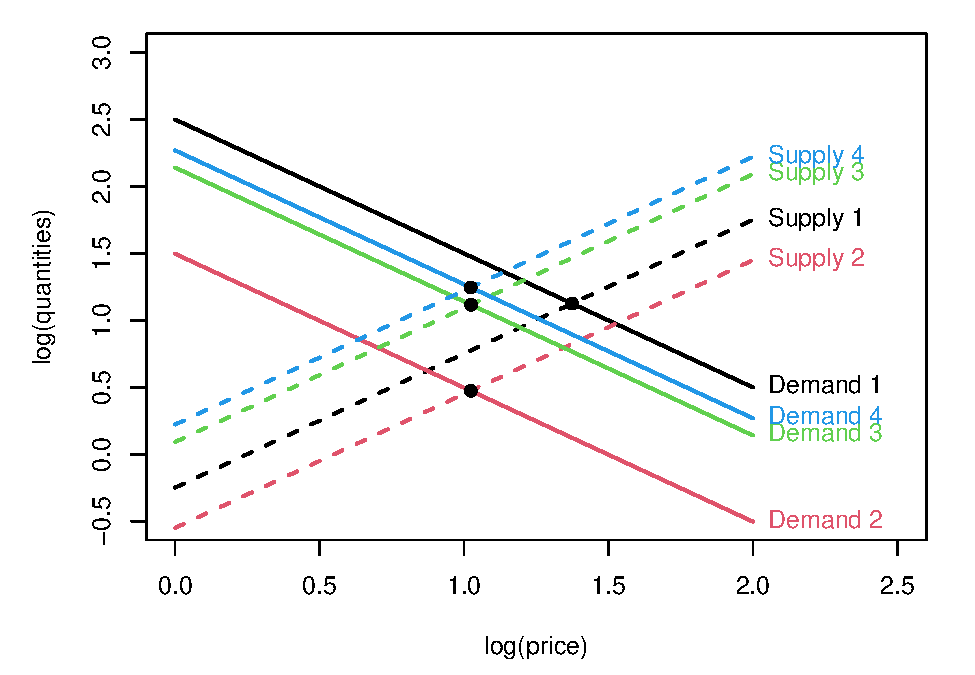
\includegraphics{_main_files/figure-latex/figureIV-1.pdf}
\caption{\label{fig:figureIV}This figure illustrates the situation prevailing when estimating a price-elasticity (and the price is endogenous).}
\end{figure}

\href{https://rpubs.com/wsundstrom/t_ivreg}{Estimation of the price elasticity of cigarette demand}. Instrument: real tax on cigarettes arising from the state's general sales tax. Presumption: in states with a larger general sales tax, cigarette prices are higher, but the general tax is not determined by other forces affecting \(\varepsilon_t^d\).

\begin{Shaded}
\begin{Highlighting}[]
\FunctionTok{data}\NormalTok{(}\StringTok{"CigarettesSW"}\NormalTok{, }\AttributeTok{package =} \StringTok{"AER"}\NormalTok{)}
\NormalTok{CigarettesSW}\SpecialCharTok{$}\NormalTok{rprice  }\OtherTok{\textless{}{-}} \FunctionTok{with}\NormalTok{(CigarettesSW, price}\SpecialCharTok{/}\NormalTok{cpi)}
\NormalTok{CigarettesSW}\SpecialCharTok{$}\NormalTok{rincome }\OtherTok{\textless{}{-}} \FunctionTok{with}\NormalTok{(CigarettesSW, income}\SpecialCharTok{/}\NormalTok{population}\SpecialCharTok{/}\NormalTok{cpi)}
\NormalTok{CigarettesSW}\SpecialCharTok{$}\NormalTok{tdiff   }\OtherTok{\textless{}{-}} \FunctionTok{with}\NormalTok{(CigarettesSW, (taxs }\SpecialCharTok{{-}}\NormalTok{ tax)}\SpecialCharTok{/}\NormalTok{cpi)}

\DocumentationTok{\#\# model }
\NormalTok{fm }\OtherTok{\textless{}{-}} \FunctionTok{ivreg}\NormalTok{(}\FunctionTok{log}\NormalTok{(packs) }\SpecialCharTok{\textasciitilde{}} \FunctionTok{log}\NormalTok{(rprice) }\SpecialCharTok{+} \FunctionTok{log}\NormalTok{(rincome) }\SpecialCharTok{|} \FunctionTok{log}\NormalTok{(rincome) }\SpecialCharTok{+}\NormalTok{ tdiff }\SpecialCharTok{+} \FunctionTok{I}\NormalTok{(tax}\SpecialCharTok{/}\NormalTok{cpi),}
            \AttributeTok{data =}\NormalTok{ CigarettesSW, }\AttributeTok{subset =}\NormalTok{ year }\SpecialCharTok{==} \StringTok{"1995"}\NormalTok{)}
\NormalTok{eq.no.IV }\OtherTok{\textless{}{-}} \FunctionTok{lm}\NormalTok{(}\FunctionTok{log}\NormalTok{(packs) }\SpecialCharTok{\textasciitilde{}} \FunctionTok{log}\NormalTok{(rprice) }\SpecialCharTok{+} \FunctionTok{log}\NormalTok{(rincome),}
               \AttributeTok{data =}\NormalTok{ CigarettesSW, }\AttributeTok{subset =}\NormalTok{ year }\SpecialCharTok{==} \StringTok{"1995"}\NormalTok{)}
\FunctionTok{summary}\NormalTok{(fm, }\AttributeTok{vcov =}\NormalTok{ sandwich, }\AttributeTok{diagnostics =} \ConstantTok{TRUE}\NormalTok{)}
\end{Highlighting}
\end{Shaded}

\begin{verbatim}
## 
## Call:
## ivreg(formula = log(packs) ~ log(rprice) + log(rincome) | log(rincome) + 
##     tdiff + I(tax/cpi), data = CigarettesSW, subset = year == 
##     "1995")
## 
## Residuals:
##        Min         1Q     Median         3Q        Max 
## -0.6006931 -0.0862222 -0.0009999  0.1164699  0.3734227 
## 
## Coefficients:
##              Estimate Std. Error t value Pr(>|t|)    
## (Intercept)    9.8950     0.9288  10.654 6.89e-14 ***
## log(rprice)   -1.2774     0.2417  -5.286 3.54e-06 ***
## log(rincome)   0.2804     0.2458   1.141     0.26    
## 
## Diagnostic tests:
##                  df1 df2 statistic p-value    
## Weak instruments   2  44   228.738  <2e-16 ***
## Wu-Hausman         1  44     3.823  0.0569 .  
## Sargan             1  NA     0.333  0.5641    
## ---
## Signif. codes:  0 '***' 0.001 '**' 0.01 '*' 0.05 '.' 0.1 ' ' 1
## 
## Residual standard error: 0.1879 on 45 degrees of freedom
## Multiple R-Squared: 0.4294,  Adjusted R-squared: 0.4041 
## Wald test: 17.25 on 2 and 45 DF,  p-value: 2.743e-06
\end{verbatim}

\begin{Shaded}
\begin{Highlighting}[]
\FunctionTok{summary}\NormalTok{(eq.no.IV)}
\end{Highlighting}
\end{Shaded}

\begin{verbatim}
## 
## Call:
## lm(formula = log(packs) ~ log(rprice) + log(rincome), data = CigarettesSW, 
##     subset = year == "1995")
## 
## Residuals:
##      Min       1Q   Median       3Q      Max 
## -0.59077 -0.07856 -0.00149  0.11860  0.35442 
## 
## Coefficients:
##              Estimate Std. Error t value Pr(>|t|)    
## (Intercept)   10.3420     1.0227  10.113 3.66e-13 ***
## log(rprice)   -1.4065     0.2514  -5.595 1.24e-06 ***
## log(rincome)   0.3439     0.2350   1.463     0.15    
## ---
## Signif. codes:  0 '***' 0.001 '**' 0.01 '*' 0.05 '.' 0.1 ' ' 1
## 
## Residual standard error: 0.1873 on 45 degrees of freedom
## Multiple R-squared:  0.4327, Adjusted R-squared:  0.4075 
## F-statistic: 17.16 on 2 and 45 DF,  p-value: 2.884e-06
\end{verbatim}

\begin{Shaded}
\begin{Highlighting}[]
\NormalTok{fm2 }\OtherTok{\textless{}{-}} \FunctionTok{ivreg}\NormalTok{(}\FunctionTok{log}\NormalTok{(packs) }\SpecialCharTok{\textasciitilde{}} \FunctionTok{log}\NormalTok{(rprice) }\SpecialCharTok{|}\NormalTok{ tdiff, }\AttributeTok{data =}\NormalTok{ CigarettesSW, }\AttributeTok{subset =}\NormalTok{ year }\SpecialCharTok{==} \StringTok{"1995"}\NormalTok{)}
\FunctionTok{anova}\NormalTok{(fm, fm2)}
\end{Highlighting}
\end{Shaded}

\begin{verbatim}
## Analysis of Variance Table
## 
## Model 1: log(packs) ~ log(rprice) + log(rincome) | log(rincome) + tdiff + 
##     I(tax/cpi)
## Model 2: log(packs) ~ log(rprice) | tdiff
##   Res.Df    RSS Df Sum of Sq      F Pr(>F)
## 1     45 1.5880                           
## 2     46 1.6668 -1 -0.078748 1.3815  0.246
\end{verbatim}

\begin{Shaded}
\begin{Highlighting}[]
\FunctionTok{library}\NormalTok{(sem)}
\FunctionTok{data}\NormalTok{(}\StringTok{"CollegeDistance"}\NormalTok{, }\AttributeTok{package =} \StringTok{"AER"}\NormalTok{)}
\NormalTok{simple.ed}\FloatTok{.1}\NormalTok{s}\OtherTok{\textless{}{-}} \FunctionTok{lm}\NormalTok{(education }\SpecialCharTok{\textasciitilde{}}\NormalTok{ urban }\SpecialCharTok{+}\NormalTok{ gender }\SpecialCharTok{+}\NormalTok{ ethnicity }\SpecialCharTok{+}\NormalTok{ unemp }\SpecialCharTok{+}\NormalTok{ distance,}
                  \AttributeTok{data =}\NormalTok{ CollegeDistance)}
\NormalTok{CollegeDistance}\SpecialCharTok{$}\NormalTok{ed.pred}\OtherTok{\textless{}{-}} \FunctionTok{predict}\NormalTok{(simple.ed}\FloatTok{.1}\NormalTok{s)}
\NormalTok{simple.ed}\FloatTok{.2}\NormalTok{s}\OtherTok{\textless{}{-}} \FunctionTok{lm}\NormalTok{(wage }\SpecialCharTok{\textasciitilde{}}\NormalTok{ urban }\SpecialCharTok{+}\NormalTok{ gender }\SpecialCharTok{+}\NormalTok{ ethnicity }\SpecialCharTok{+}\NormalTok{ unemp }\SpecialCharTok{+}\NormalTok{ ed.pred ,}
                  \AttributeTok{data =}\NormalTok{ CollegeDistance)}

\NormalTok{simple.comp}\OtherTok{\textless{}{-}} \FunctionTok{encomptest}\NormalTok{(wage }\SpecialCharTok{\textasciitilde{}}\NormalTok{ urban }\SpecialCharTok{+}\NormalTok{ gender }\SpecialCharTok{+}\NormalTok{ ethnicity }\SpecialCharTok{+}\NormalTok{ unemp }\SpecialCharTok{+}\NormalTok{ ed.pred ,}
\NormalTok{                         wage }\SpecialCharTok{\textasciitilde{}}\NormalTok{ urban }\SpecialCharTok{+}\NormalTok{ gender }\SpecialCharTok{+}\NormalTok{ ethnicity }\SpecialCharTok{+}\NormalTok{ unemp }\SpecialCharTok{+}\NormalTok{ education ,}
                         \AttributeTok{data =}\NormalTok{ CollegeDistance)}
\NormalTok{fsttest}\OtherTok{\textless{}{-}} \FunctionTok{encomptest}\NormalTok{(education }\SpecialCharTok{\textasciitilde{}}\NormalTok{ tuition }\SpecialCharTok{+}\NormalTok{ gender }\SpecialCharTok{+}\NormalTok{ ethnicity }\SpecialCharTok{+}\NormalTok{ urban ,}
\NormalTok{                     education }\SpecialCharTok{\textasciitilde{}}\NormalTok{ distance ,}
                     \AttributeTok{data =}\NormalTok{ CollegeDistance)}

\NormalTok{eqOLS }\OtherTok{\textless{}{-}} \FunctionTok{lm}\NormalTok{(wage }\SpecialCharTok{\textasciitilde{}}\NormalTok{ urban }\SpecialCharTok{+}\NormalTok{ gender }\SpecialCharTok{+}\NormalTok{ ethnicity }\SpecialCharTok{+}\NormalTok{ unemp }\SpecialCharTok{+}\NormalTok{ education,}
            \AttributeTok{data=}\NormalTok{CollegeDistance)}

\FunctionTok{summary}\NormalTok{(eqOLS)}
\end{Highlighting}
\end{Shaded}

\begin{verbatim}
## 
## Call:
## lm(formula = wage ~ urban + gender + ethnicity + unemp + education, 
##     data = CollegeDistance)
## 
## Residuals:
##     Min      1Q  Median      3Q     Max 
## -3.3484 -0.8408  0.1808  0.8119  3.9875 
## 
## Coefficients:
##                    Estimate Std. Error t value Pr(>|t|)    
## (Intercept)        8.641490   0.157008  55.039   <2e-16 ***
## urbanyes           0.070117   0.044727   1.568   0.1170    
## genderfemale      -0.085242   0.037069  -2.300   0.0215 *  
## ethnicityafam     -0.556056   0.052167 -10.659   <2e-16 ***
## ethnicityhispanic -0.544007   0.048670 -11.177   <2e-16 ***
## unemp              0.133101   0.006711  19.834   <2e-16 ***
## education          0.005369   0.010362   0.518   0.6044    
## ---
## Signif. codes:  0 '***' 0.001 '**' 0.01 '*' 0.05 '.' 0.1 ' ' 1
## 
## Residual standard error: 1.268 on 4732 degrees of freedom
## Multiple R-squared:  0.1098, Adjusted R-squared:  0.1087 
## F-statistic: 97.27 on 6 and 4732 DF,  p-value: < 2.2e-16
\end{verbatim}

\begin{Shaded}
\begin{Highlighting}[]
\FunctionTok{summary}\NormalTok{(simple.ed}\FloatTok{.2}\NormalTok{s)}
\end{Highlighting}
\end{Shaded}

\begin{verbatim}
## 
## Call:
## lm(formula = wage ~ urban + gender + ethnicity + unemp + ed.pred, 
##     data = CollegeDistance)
## 
## Residuals:
##     Min      1Q  Median      3Q     Max 
## -3.1692 -0.8294  0.1502  0.8482  3.9537 
## 
## Coefficients:
##                    Estimate Std. Error t value Pr(>|t|)    
## (Intercept)       -0.359032   1.412087  -0.254  0.79931    
## urbanyes           0.046144   0.044691   1.033  0.30188    
## genderfemale      -0.070753   0.036978  -1.913  0.05576 .  
## ethnicityafam     -0.227240   0.072984  -3.114  0.00186 ** 
## ethnicityhispanic -0.351291   0.057021  -6.161 7.84e-10 ***
## unemp              0.139163   0.006748  20.622  < 2e-16 ***
## ed.pred            0.647099   0.100592   6.433 1.38e-10 ***
## ---
## Signif. codes:  0 '***' 0.001 '**' 0.01 '*' 0.05 '.' 0.1 ' ' 1
## 
## Residual standard error: 1.263 on 4732 degrees of freedom
## Multiple R-squared:  0.1175, Adjusted R-squared:  0.1163 
## F-statistic:   105 on 6 and 4732 DF,  p-value: < 2.2e-16
\end{verbatim}

\begin{Shaded}
\begin{Highlighting}[]
\NormalTok{eqTSLS }\OtherTok{\textless{}{-}} \FunctionTok{tsls}\NormalTok{(wage }\SpecialCharTok{\textasciitilde{}}\NormalTok{ urban }\SpecialCharTok{+}\NormalTok{ gender }\SpecialCharTok{+}\NormalTok{ ethnicity }\SpecialCharTok{+}\NormalTok{ unemp }\SpecialCharTok{+}\NormalTok{ education,}
               \SpecialCharTok{\textasciitilde{}}\NormalTok{ urban }\SpecialCharTok{+}\NormalTok{ gender }\SpecialCharTok{+}\NormalTok{ ethnicity }\SpecialCharTok{+}\NormalTok{ unemp }\SpecialCharTok{+}\NormalTok{ distance,}
               \AttributeTok{data=}\NormalTok{CollegeDistance)}

\NormalTok{eqTSLS }\OtherTok{\textless{}{-}} \FunctionTok{ivreg}\NormalTok{(wage }\SpecialCharTok{\textasciitilde{}}\NormalTok{ urban }\SpecialCharTok{+}\NormalTok{ gender }\SpecialCharTok{+}\NormalTok{ ethnicity }\SpecialCharTok{+}\NormalTok{ unemp }\SpecialCharTok{+}\NormalTok{ education}\SpecialCharTok{|}
\NormalTok{                  urban }\SpecialCharTok{+}\NormalTok{ gender }\SpecialCharTok{+}\NormalTok{ ethnicity }\SpecialCharTok{+}\NormalTok{ unemp }\SpecialCharTok{+}\NormalTok{ distance,}
                \AttributeTok{data=}\NormalTok{CollegeDistance)}

\FunctionTok{summary}\NormalTok{(eqTSLS, }\AttributeTok{vcov =}\NormalTok{ sandwich, }\AttributeTok{diagnostics =} \ConstantTok{TRUE}\NormalTok{)}
\end{Highlighting}
\end{Shaded}

\begin{verbatim}
## 
## Call:
## ivreg(formula = wage ~ urban + gender + ethnicity + unemp + education | 
##     urban + gender + ethnicity + unemp + distance, data = CollegeDistance)
## 
## Residuals:
##      Min       1Q   Median       3Q      Max 
## -5.20896 -1.14578 -0.02361  1.33303  4.77571 
## 
## Coefficients:
##                   Estimate Std. Error t value Pr(>|t|)    
## (Intercept)       -0.35903    1.91755  -0.187   0.8515    
## urbanyes           0.04614    0.05926   0.779   0.4362    
## genderfemale      -0.07075    0.04974  -1.422   0.1550    
## ethnicityafam     -0.22724    0.09539  -2.382   0.0172 *  
## ethnicityhispanic -0.35129    0.07577  -4.636 3.64e-06 ***
## unemp              0.13916    0.00934  14.899  < 2e-16 ***
## education          0.64710    0.13691   4.727 2.35e-06 ***
## 
## Diagnostic tests:
##                   df1  df2 statistic  p-value    
## Weak instruments    1 4732     50.19 1.60e-12 ***
## Wu-Hausman          1 4731     40.30 2.38e-10 ***
## Sargan              0   NA        NA       NA    
## ---
## Signif. codes:  0 '***' 0.001 '**' 0.01 '*' 0.05 '.' 0.1 ' ' 1
## 
## Residual standard error: 1.706 on 4732 degrees of freedom
## Multiple R-Squared: -0.6118, Adjusted R-squared: -0.6138 
## Wald test: 57.08 on 6 and 4732 DF,  p-value: < 2.2e-16
\end{verbatim}

\hypertarget{general-regression-model}{%
\section{General Regression Model}\label{general-regression-model}}

We want to relax the assumption according to which the disturbances are uncorrelated with each other (Hypothesis @ref(hyp:noncorrel\_resid)) or the homoskedasticity Hypothesis \ref{hyp:homoskedasticity}.

We replace the latter two assumptions by the general formulation:
\begin{eqnarray}
\mathbb{E}(\boldsymbol\varepsilon \boldsymbol\varepsilon'| \mathbf{X}) &=& \boldsymbol\Sigma. \label{eq:assumGLS2}
\end{eqnarray}

Note that Eq. (\eqref{eq:assumGLS2}) is more general than Hypothesis \ref{hyp:homoskedasticity} and @ref(hyp:noncorrel\_resid) because the diagonal entries of \(\boldsymbol\Sigma\) may be different (not the case under Hypothesis \ref{hyp:homoskedasticity}), and the non-diagonal entries of \(\boldsymbol\Sigma\) can be \(\ne 0\) (contrary to Hypothesis \ref{hyp:noncorrelResid}).

\begin{definition}
\protect\hypertarget{def:GRM}{}\label{def:GRM}Hypothesis \ref{hyp:fullrank} and \ref{hyp:exogeneity}, together with Eq. \eqref{eq:assumGLS2}, form the \textbf{General Regression Model} (GRM) framework.
\end{definition}

Note that a regression model where Hypotheses \ref{hyp:fullrank} to \ref{hyp:noncorrelResid} hold is a specific case of the GRM framework.

The GRM context notably allows to model \textbf{heteroskedasticity} and \textbf{autocorrelation}.

\begin{itemize}
\tightlist
\item
  Heteroskedasticity:
  \begin{equation}
  \boldsymbol\Sigma = \left[  \begin{array}{cccc}
  \sigma_1^2 & 0 & \dots & 0 \\
  0 & \sigma_2^2 &  & 0 \\
  \vdots && \ddots& \vdots \\
  0 & \dots & 0 & \sigma_n^2
  \end{array} \right]. \label{eq:heteroskedasticity}
  \end{equation}
\item
  Autocorrelation:
  \begin{equation}
  \boldsymbol\Sigma = \sigma^2 \left[ \begin{array}{cccc}
  1 & \rho_{2,1} & \dots & \rho_{n,1} \\
  \rho_{2,1} & 1 &  & \vdots \\
  \vdots && \ddots& \rho_{n,n-1} \\
  \rho_{n,1} & \rho_{n,2} & \dots & 1
  \end{array} \right]. \label{eq:autocorrelation}
  \end{equation}
\end{itemize}

\begin{example}
\protect\hypertarget{exm:autocorrelaaa}{}\label{exm:autocorrelaaa}Autocorrelation is, in particular, a recurrent problem when time-series data are used (see Section \ref{section:TS}).

In a time-series context, subscript \(i\) refers to a date. Assume for instance that:
\begin{equation}\label{eq:usual}
y_i = \mathbf{x}_i' \boldsymbol\beta + \varepsilon_i
\end{equation}
with
\begin{equation}\label{eq:usual2}
\varepsilon_i = \rho \varepsilon_{i-1} + v_i, \quad v_i \sim \mathcal{N}(0,\sigma_v^2).
\end{equation}
In this case, we are in the GRM context, with:
\begin{equation}\label{eq:SigmaAutocorrel}
\boldsymbol\Sigma =\frac{ \sigma_v^2}{1 - \rho^2} \left[    \begin{array}{cccc}
1 & \rho & \dots & \rho^{n-1} \\
\rho & 1 &  & \vdots \\
\vdots && \ddots& \rho \\
\rho^{n-1} & \rho^{n-2} & \dots & 1
\end{array} \right].
\end{equation}
\end{example}

\hypertarget{generalized-least-squares}{%
\subsection{Generalized Least Squares}\label{generalized-least-squares}}

Assume \(\boldsymbol\Sigma\) is known (``feasible GLS'\,'). Because \(\boldsymbol\Sigma\) is symmetric positive, it admits a spectral decomposition of the form \(\boldsymbol\Sigma = \mathbf{C} \boldsymbol\Lambda \mathbf{C}'\), where \(\mathbf{C}\) is an orthogonal matrix (i.e.~\(\mathbf{C}\mathbf{C}'=Id\)) and \(\boldsymbol\Lambda\) is a diagonal matrix (the diagonal entries are the eigenvalues of \(\boldsymbol\Sigma\)).

We have \(\boldsymbol\Sigma = (\mathbf{P}\mathbf{P}')^{-1}\) with \(\mathbf{P} = \mathbf{C}\boldsymbol\Lambda^{-1/2}\).

Consider the transformed model:
\[
\mathbf{P}'\mathbf{y} = \mathbf{P}'\mathbf{X}\boldsymbol\beta + \mathbf{P}'\boldsymbol\varepsilon \quad \mbox{or} \quad \mathbf{y}^* = \mathbf{X}^*\boldsymbol\beta + \boldsymbol\varepsilon^*.
\]
The variance of \(\boldsymbol\varepsilon^*\) is \(\mathbf{I}\). In the transformed model, OLS is BLUE (Gauss-Markow Theorem \ref{thm:GaussMarkov}).

The \textbf{Generalized least squares} estimator of \(\boldsymbol\beta\) is:
\begin{equation}
\boxed{\mathbf{b}_{GLS} = (\mathbf{X}'\boldsymbol\Sigma^{-1}\mathbf{X})^{-1}\mathbf{X}'\boldsymbol\Sigma^{-1}\mathbf{y}}.\label{eq:betaGLS}
\end{equation}
We have:
\[
\mathbb{V}ar(\mathbf{b}_{GLS}|\mathbf{X}) = (\mathbf{X}'\boldsymbol\Sigma^{-1}\mathbf{X})^{-1}.
\]

When \(\boldsymbol\Sigma\) is unknown, the GLS estimator is said to be \emph{infeasible}. Some structure is required. Assume \(\boldsymbol\Sigma\) admits a parametric form \(\boldsymbol\Sigma(\theta)\). The estimation becomes \emph{feasible} (FGLS) if one replaces \(\boldsymbol\Sigma(\theta)\) by \(\boldsymbol\Sigma(\hat\theta)\).

If \(\hat\theta\) is a consistent estimator of \(\theta\), then the FGLS is asymptotically efficient (see Example \ref{exm:autocorrelaa}).

By contrast, when \(\boldsymbol\Sigma\) has no obvious structure: the OLS (or IV) is the only estimator available. It remains unbiased, consistent, and asymptotically normally distributed, but not efficient. Standard inference procedures are not appropriate any longer.

Autocorrelation in the time-series context. Consider the case presented in Example \ref{exm:autocorrelaaa}. Because the OLS estimate \(\mathbf{b}\) of \(\boldsymbol\beta\) is consistent, the estimates \(e_i\)s of the \(\varepsilon_i\)s also are. Consistent estimators of \(\rho\) and \(\sigma_v\) are then obtained by regressing the \(e_i\)s on the \(e_{i-1}\)s. Using these estimates in Eq. \eqref{eq:SigmaAutocorrel} provides a consistent estimate of \(\boldsymbol\Sigma\).

See \href{https://www.tandfonline.com/doi/abs/10.1080/01621459.1949.10483290}{Cochrane and Orcutt (2012)}.

\begin{center}\rule{0.5\linewidth}{0.5pt}\end{center}

\begin{proposition}
\protect\hypertarget{prp:AsymptOLSGRM}{}\label{prp:AsymptOLSGRM}Conditionally on \(\mathbf{X}\), we have:
\begin{equation}
\mathbb{V}ar(\mathbf{b}|\mathbf{X}) = \frac{1}{n}\left(\frac{1}{n}\mathbf{X}'\mathbf{X}\right)^{-1}\left(\frac{1}{n}\mathbf{X}'\boldsymbol\Sigma\mathbf{X}\right)\left(\frac{1}{n}\mathbf{X}'\mathbf{X}\right)^{-1}.\label{eq:xsx}
\end{equation}
Under Hypothesis \ref{hyp:normality}, since \(\mathbf{b}\) is linear in \(\boldsymbol\varepsilon\), we have:
\begin{equation}
\mathbf{b}|\mathbf{X} \sim \mathcal{N}\left(\boldsymbol\beta,\left(\mathbf{X}'\mathbf{X}\right)^{-1}\left(\mathbf{X}'\boldsymbol\Sigma\mathbf{X}\right)\left(\mathbf{X}'\mathbf{X}\right)^{-1}\right).
\end{equation}
\end{proposition}

\begin{center}\rule{0.5\linewidth}{0.5pt}\end{center}

Note that the variance of the estimator is not \(\sigma^2 (\mathbf{X}'\mathbf{X})^{-1}\) any more, so using \(s^2 (\mathbf{X}'\mathbf{X})^{-1}\) for inference may be misleading.

\begin{center}\rule{0.5\linewidth}{0.5pt}\end{center}

\begin{proposition}
\protect\hypertarget{prp:XXX}{}\label{prp:XXX}If \(\mbox{plim }(\mathbf{X}'\mathbf{X}/n)\) and \(\mbox{plim }(\mathbf{X}'\boldsymbol\Sigma\mathbf{X}/n)\) are finite positive definite matrices, then \(\mbox{plim }(\mathbf{b})=\boldsymbol\beta\).
\end{proposition}

\begin{center}\rule{0.5\linewidth}{0.5pt}\end{center}

\begin{proof}
We have \(\mathbb{V}ar(\mathbf{b})=\mathbb{E}[\mathbb{V}ar(\mathbf{b}|\mathbf{X})]+\mathbb{V}ar[\mathbb{E}(\mathbf{b}|\mathbf{X})]\). Since \(\mathbb{E}(\mathbf{b}|\mathbf{X})=\boldsymbol\beta\), \(\mathbb{V}ar[\mathbb{E}(\mathbf{b}|\mathbf{X})]=0\). Eq. \eqref{eq:xsx} implies that \(\mathbb{V}ar(\mathbf{b}|\mathbf{X}) \rightarrow 0\). Hence \(\mathbf{b}\) converges in mean square and therefore in probability. \(\square\)
\end{proof}

\begin{center}\rule{0.5\linewidth}{0.5pt}\end{center}

\begin{proposition}
\protect\hypertarget{prp:AsymptGRM}{}\label{prp:AsymptGRM}If \(Q_{xx}=\mbox{plim }(\mathbf{X}'\mathbf{X}/n)\) and \(Q_{x\boldsymbol\Sigma x}=\mbox{plim }(\mathbf{X}'\boldsymbol\Sigma\mathbf{X}/n)\) are finite positive definite matrices, then:
\[
\sqrt{n}(\mathbf{b}-\boldsymbol\beta) \overset{d}{\rightarrow} \mathcal{N}(0,Q_{xx}^{-1}Q_{x\boldsymbol\Sigma x}Q_{xx}^{-1}).
\]
\end{proposition}

\begin{center}\rule{0.5\linewidth}{0.5pt}\end{center}

\begin{center}\rule{0.5\linewidth}{0.5pt}\end{center}

\begin{proposition}
\protect\hypertarget{prp:AsymptIVGRM}{}\label{prp:AsymptIVGRM}If regressors and IV variables are ``well-behaved'\,', then:
\[
\mathbf{b}_{iv} \overset{a}{\sim} \mathcal{N}(\boldsymbol\beta,\mathbf{V}_{iv}),
\]
where
\[
\mathbf{V}_{iv} = \frac{1}{n}(\mathbf{Q}^*)\mbox{ plim }\left( \frac{1}{n} \mathbf{Z}'\boldsymbol\Sigma \mathbf{Z}\right)(\mathbf{Q}^*)',
\]
with
\[
\mathbf{Q}^* = [\mathbf{Q}_{xz}\mathbf{Q}_{zz}^{-1}\mathbf{Q}_{zx}]^{-1}\mathbf{Q}_{xz}\mathbf{Q}_{zz}^{-1}.
\]
\end{proposition}

\begin{center}\rule{0.5\linewidth}{0.5pt}\end{center}

For practical purposes, one needs to have estimates of \(\boldsymbol\Sigma\) in Props. \ref{prp:AsymptOLSGRM}, \ref{prp:AsymptGRM} or \ref{prp:AsymptIVGRM}.

Idea: instead of estimating \(\boldsymbol\Sigma\) (dimension \(n \times n\)) directly, one can estimate \(\frac{1}{n}\mathbf{X}'\boldsymbol\Sigma\mathbf{X}\), of dimension \(K \times K\) (or \(\frac{1}{n}\mathbf{Z}'\boldsymbol\Sigma\mathbf{Z}\) in the IV case). Indeed, this is this expression (\(\mathbf{X}'\boldsymbol\Sigma\mathbf{X}\)) that eventually appears in the formulas -- for instance in Eq. \eqref{eq:xsx}.

We have:
\begin{equation}
\frac{1}{n}\mathbf{X}'\boldsymbol\Sigma\mathbf{X} = \frac{1}{n}\sum_{i=1}^{n}\sum_{j=1}^{n}\sigma_{i,j}\mathbf{x}_i\mathbf{x}'_j. \label{eq:GeneralXSigmaX}
\end{equation}

\textbf{Robust estimation of asymptotic covariance matrices} look for estimates of the previous matrix. Their computation is based on the fact that if \(\mathbf{b}\) is consistent, then the \(e_i\)s are consistent (pointwise) estimators of the \(\varepsilon_i\)s.

\begin{example}
\protect\hypertarget{exm:heteroskedasticity}{}\label{exm:heteroskedasticity}\textbf{Heteroskedasticity}.

This is the case of Eq. \eqref{eq:heteroskedasticity}.

We then need to estimate \(\frac{1}{n}\sum_{i=1}^{n}\sigma_{i}^2\mathbf{x}_i\mathbf{x}'_i\). \href{http://www.jstor.org/stable/1912934}{White (1980)}: Under general conditions:
\begin{equation}
\mbox{plim}\left( \frac{1}{n}\sum_{i=1}^{n}\sigma_{i}^2\mathbf{x}_i\mathbf{x}'_i \right) = 
\mbox{plim}\left( \frac{1}{n}\sum_{i=1}^{n}e_{i}^2\mathbf{x}_i\mathbf{x}'_i \right). \label{eq:white}
\end{equation}
The estimator of \(\frac{1}{n}\mathbf{X}'\boldsymbol\Sigma\mathbf{X}\) therefore is:
\[
\frac{1}{n}\mathbf{X}'\mathbf{E}^2\mathbf{X},
\]
where \(\mathbf{E}\) is an \(n \times n\) diagonal matrix whose diagonal elements are the estimated residuals \(e_i\).

Illustration: Figure \ref{fig:exmpSalarayPhD}.
\end{example}

Let us illustrate the influence of heteroskedasticity using simulations.

We consider the following model:
\[
y_i = x_i + \varepsilon_i, \quad \varepsilon_i \sim \mathcal{N}(0,x_i^2).
\]
where the \(x_i\)s are i.i.d. \(t(4)\).

Here is a simulated sample (\(n=200\)) of this model:

\begin{Shaded}
\begin{Highlighting}[]
\NormalTok{n }\OtherTok{\textless{}{-}} \DecValTok{200}
\NormalTok{x }\OtherTok{\textless{}{-}} \FunctionTok{rt}\NormalTok{(n,}\AttributeTok{df=}\DecValTok{5}\NormalTok{)}
\NormalTok{y }\OtherTok{\textless{}{-}}\NormalTok{ x }\SpecialCharTok{+}\NormalTok{ x}\SpecialCharTok{*}\FunctionTok{rnorm}\NormalTok{(n)}
\FunctionTok{plot}\NormalTok{(x,y,}\AttributeTok{pch=}\DecValTok{19}\NormalTok{)}
\end{Highlighting}
\end{Shaded}

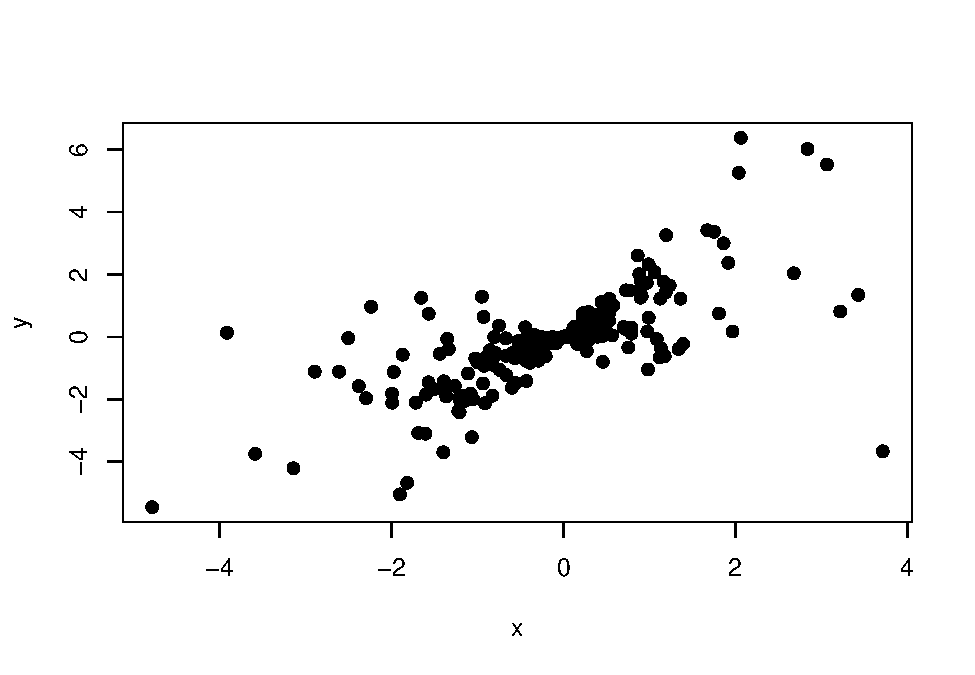
\includegraphics{_main_files/figure-latex/simulHeterosk-1.pdf}

We simulate 1000 samples of the same model with \(n=200\). For each sample, we compute the OLS estimate of \(\beta\) (=1). Using these 1000 estimates of \(b\), we construct an approximated \emph{(kernel-based) distribution of this OLS estimator} (in red on the figure).

For each of the 1000 OLS estimations, we employ \emph{the standard OLS variance formula (\(s^2 (\mathbf{X}'\mathbf{X})^{-1}\))} to estimate the variance of \(b\). The blue curve is a normal distribution centred on 1 and whose variance is the average of the 1000 previous variance estimates.

The variance of the simulated \(b\) is of 0.040 (that is the \emph{true} one); the average of the estimated variances based on the standard OLS formula is of 0.005 (\emph{bad} estimate); the average of the estimated variances based on the White robust covariance matrix is of 0.030 (better estimate).

The standard OLS formula for the variance of \(b\) overestimates the precision of this estimator.

For almost 50\% of the simulations, 1 is not included in the 95\% confidence interval of \(\beta\) when the computation of the interval is based on the standard OLS formula for the variance of \(b\).

When the White robust covariance matrix is used, 1 is not in the 95\% confidence interval of \(\beta\) for less than 10\% of the simulations.

\begin{Shaded}
\begin{Highlighting}[]
\NormalTok{n }\OtherTok{\textless{}{-}} \DecValTok{200}
\NormalTok{N }\OtherTok{\textless{}{-}} \DecValTok{1000}
\NormalTok{XX }\OtherTok{\textless{}{-}} \FunctionTok{matrix}\NormalTok{(}\FunctionTok{rt}\NormalTok{(n}\SpecialCharTok{*}\NormalTok{N,}\AttributeTok{df=}\DecValTok{5}\NormalTok{),n,N)}
\NormalTok{YY }\OtherTok{\textless{}{-}} \FunctionTok{matrix}\NormalTok{(XX }\SpecialCharTok{+}\NormalTok{ XX}\SpecialCharTok{*}\FunctionTok{rnorm}\NormalTok{(n),n,N)}
\NormalTok{all\_b       }\OtherTok{\textless{}{-}} \ConstantTok{NULL}
\NormalTok{all\_V\_OLS   }\OtherTok{\textless{}{-}} \ConstantTok{NULL}
\NormalTok{all\_V\_White }\OtherTok{\textless{}{-}} \ConstantTok{NULL}
\ControlFlowTok{for}\NormalTok{(j }\ControlFlowTok{in} \DecValTok{1}\SpecialCharTok{:}\NormalTok{N)\{}
\NormalTok{  Y }\OtherTok{\textless{}{-}} \FunctionTok{matrix}\NormalTok{(YY[,j],}\AttributeTok{ncol=}\DecValTok{1}\NormalTok{)}
\NormalTok{  X }\OtherTok{\textless{}{-}} \FunctionTok{matrix}\NormalTok{(XX[,j],}\AttributeTok{ncol=}\DecValTok{1}\NormalTok{)}
\NormalTok{  b }\OtherTok{\textless{}{-}} \FunctionTok{solve}\NormalTok{(}\FunctionTok{t}\NormalTok{(X)}\SpecialCharTok{\%*\%}\NormalTok{X) }\SpecialCharTok{\%*\%} \FunctionTok{t}\NormalTok{(X)}\SpecialCharTok{\%*\%}\NormalTok{Y}
\NormalTok{  e }\OtherTok{\textless{}{-}}\NormalTok{ Y }\SpecialCharTok{{-}}\NormalTok{ X }\SpecialCharTok{\%*\%}\NormalTok{ b}
\NormalTok{  S }\OtherTok{\textless{}{-}} \DecValTok{1}\SpecialCharTok{/}\NormalTok{n }\SpecialCharTok{*} \FunctionTok{t}\NormalTok{(X) }\SpecialCharTok{\%*\%} \FunctionTok{diag}\NormalTok{(}\FunctionTok{c}\NormalTok{(e}\SpecialCharTok{\^{}}\DecValTok{2}\NormalTok{)) }\SpecialCharTok{\%*\%}\NormalTok{ X}
\NormalTok{  V\_OLS   }\OtherTok{\textless{}{-}} \FunctionTok{solve}\NormalTok{(}\FunctionTok{t}\NormalTok{(X)}\SpecialCharTok{\%*\%}\NormalTok{X) }\SpecialCharTok{*} \FunctionTok{var}\NormalTok{(e)}
\NormalTok{  V\_White }\OtherTok{\textless{}{-}} \DecValTok{1}\SpecialCharTok{/}\NormalTok{n }\SpecialCharTok{*}\NormalTok{ (}\FunctionTok{solve}\NormalTok{(}\DecValTok{1}\SpecialCharTok{/}\NormalTok{n}\SpecialCharTok{*}\FunctionTok{t}\NormalTok{(X)}\SpecialCharTok{\%*\%}\NormalTok{X)) }\SpecialCharTok{\%*\%}\NormalTok{ S }\SpecialCharTok{\%*\%}\NormalTok{ (}\FunctionTok{solve}\NormalTok{(}\DecValTok{1}\SpecialCharTok{/}\NormalTok{n}\SpecialCharTok{*}\FunctionTok{t}\NormalTok{(X)}\SpecialCharTok{\%*\%}\NormalTok{X))}
  
\NormalTok{  all\_b       }\OtherTok{\textless{}{-}} \FunctionTok{c}\NormalTok{(all\_b,b)}
\NormalTok{  all\_V\_OLS   }\OtherTok{\textless{}{-}} \FunctionTok{c}\NormalTok{(all\_V\_OLS,V\_OLS)}
\NormalTok{  all\_V\_White }\OtherTok{\textless{}{-}} \FunctionTok{c}\NormalTok{(all\_V\_White,V\_White)}
\NormalTok{\}}
\FunctionTok{plot}\NormalTok{(}\FunctionTok{density}\NormalTok{(all\_b))}
\FunctionTok{abline}\NormalTok{(}\AttributeTok{v=}\FunctionTok{mean}\NormalTok{(all\_b),}\AttributeTok{lty=}\DecValTok{2}\NormalTok{)}
\FunctionTok{abline}\NormalTok{(}\AttributeTok{v=}\DecValTok{1}\NormalTok{)}
\NormalTok{x }\OtherTok{\textless{}{-}} \FunctionTok{seq}\NormalTok{(}\DecValTok{0}\NormalTok{,}\DecValTok{2}\NormalTok{,}\AttributeTok{by=}\NormalTok{.}\DecValTok{01}\NormalTok{)}
\FunctionTok{lines}\NormalTok{(x,}\FunctionTok{dnorm}\NormalTok{(x,}\AttributeTok{mean =} \DecValTok{1}\NormalTok{,}\AttributeTok{sd =} \FunctionTok{mean}\NormalTok{(}\FunctionTok{sqrt}\NormalTok{(all\_V\_OLS))),}\AttributeTok{col=}\StringTok{"blue"}\NormalTok{)}
\FunctionTok{lines}\NormalTok{(x,}\FunctionTok{dnorm}\NormalTok{(x,}\AttributeTok{mean =} \DecValTok{1}\NormalTok{,}\AttributeTok{sd =} \FunctionTok{mean}\NormalTok{(}\FunctionTok{sqrt}\NormalTok{(all\_V\_White))),}\AttributeTok{col=}\StringTok{"red"}\NormalTok{)}
\end{Highlighting}
\end{Shaded}

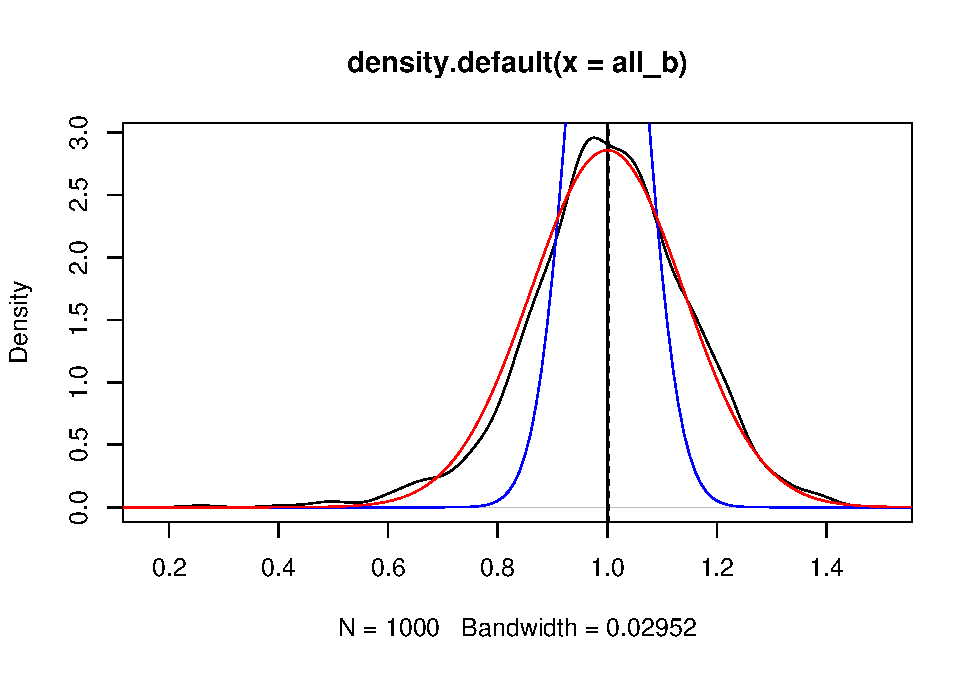
\includegraphics{_main_files/figure-latex/simulHeterosk2-1.pdf}

\hypertarget{appendix}{%
\chapter{Appendix}\label{appendix}}

\hypertarget{statitical-tables}{%
\section{Statitical Tables}\label{statitical-tables}}

\begin{table}

\caption{\label{tab:Normal}Quantiles of the $\mathcal{N}(0,1)$ distribution. If $a$ and $b$ are respectively the row and column number; then the corresponding cell gives $\mathbb{P}(0<X\le a+b)$, where $X \sim \mathcal{N}(0,1)$.}
\centering
\begin{tabular}[t]{l|r|r|r|r|r|r|r|r|r|r}
\hline
  & 0 & 0.01 & 0.02 & 0.03 & 0.04 & 0.05 & 0.06 & 0.07 & 0.08 & 0.09\\
\hline
0 & 0.5000 & 0.6179 & 0.7257 & 0.8159 & 0.8849 & 0.9332 & 0.9641 & 0.9821 & 0.9918 & 0.9965\\
\hline
0.1 & 0.5040 & 0.6217 & 0.7291 & 0.8186 & 0.8869 & 0.9345 & 0.9649 & 0.9826 & 0.9920 & 0.9966\\
\hline
0.2 & 0.5080 & 0.6255 & 0.7324 & 0.8212 & 0.8888 & 0.9357 & 0.9656 & 0.9830 & 0.9922 & 0.9967\\
\hline
0.3 & 0.5120 & 0.6293 & 0.7357 & 0.8238 & 0.8907 & 0.9370 & 0.9664 & 0.9834 & 0.9925 & 0.9968\\
\hline
0.4 & 0.5160 & 0.6331 & 0.7389 & 0.8264 & 0.8925 & 0.9382 & 0.9671 & 0.9838 & 0.9927 & 0.9969\\
\hline
0.5 & 0.5199 & 0.6368 & 0.7422 & 0.8289 & 0.8944 & 0.9394 & 0.9678 & 0.9842 & 0.9929 & 0.9970\\
\hline
0.6 & 0.5239 & 0.6406 & 0.7454 & 0.8315 & 0.8962 & 0.9406 & 0.9686 & 0.9846 & 0.9931 & 0.9971\\
\hline
0.7 & 0.5279 & 0.6443 & 0.7486 & 0.8340 & 0.8980 & 0.9418 & 0.9693 & 0.9850 & 0.9932 & 0.9972\\
\hline
0.8 & 0.5319 & 0.6480 & 0.7517 & 0.8365 & 0.8997 & 0.9429 & 0.9699 & 0.9854 & 0.9934 & 0.9973\\
\hline
0.9 & 0.5359 & 0.6517 & 0.7549 & 0.8389 & 0.9015 & 0.9441 & 0.9706 & 0.9857 & 0.9936 & 0.9974\\
\hline
1 & 0.5398 & 0.6554 & 0.7580 & 0.8413 & 0.9032 & 0.9452 & 0.9713 & 0.9861 & 0.9938 & 0.9974\\
\hline
1.1 & 0.5438 & 0.6591 & 0.7611 & 0.8438 & 0.9049 & 0.9463 & 0.9719 & 0.9864 & 0.9940 & 0.9975\\
\hline
1.2 & 0.5478 & 0.6628 & 0.7642 & 0.8461 & 0.9066 & 0.9474 & 0.9726 & 0.9868 & 0.9941 & 0.9976\\
\hline
1.3 & 0.5517 & 0.6664 & 0.7673 & 0.8485 & 0.9082 & 0.9484 & 0.9732 & 0.9871 & 0.9943 & 0.9977\\
\hline
1.4 & 0.5557 & 0.6700 & 0.7704 & 0.8508 & 0.9099 & 0.9495 & 0.9738 & 0.9875 & 0.9945 & 0.9977\\
\hline
1.5 & 0.5596 & 0.6736 & 0.7734 & 0.8531 & 0.9115 & 0.9505 & 0.9744 & 0.9878 & 0.9946 & 0.9978\\
\hline
1.6 & 0.5636 & 0.6772 & 0.7764 & 0.8554 & 0.9131 & 0.9515 & 0.9750 & 0.9881 & 0.9948 & 0.9979\\
\hline
1.7 & 0.5675 & 0.6808 & 0.7794 & 0.8577 & 0.9147 & 0.9525 & 0.9756 & 0.9884 & 0.9949 & 0.9979\\
\hline
1.8 & 0.5714 & 0.6844 & 0.7823 & 0.8599 & 0.9162 & 0.9535 & 0.9761 & 0.9887 & 0.9951 & 0.9980\\
\hline
1.9 & 0.5753 & 0.6879 & 0.7852 & 0.8621 & 0.9177 & 0.9545 & 0.9767 & 0.9890 & 0.9952 & 0.9981\\
\hline
2 & 0.5793 & 0.6915 & 0.7881 & 0.8643 & 0.9192 & 0.9554 & 0.9772 & 0.9893 & 0.9953 & 0.9981\\
\hline
2.1 & 0.5832 & 0.6950 & 0.7910 & 0.8665 & 0.9207 & 0.9564 & 0.9778 & 0.9896 & 0.9955 & 0.9982\\
\hline
2.2 & 0.5871 & 0.6985 & 0.7939 & 0.8686 & 0.9222 & 0.9573 & 0.9783 & 0.9898 & 0.9956 & 0.9982\\
\hline
2.3 & 0.5910 & 0.7019 & 0.7967 & 0.8708 & 0.9236 & 0.9582 & 0.9788 & 0.9901 & 0.9957 & 0.9983\\
\hline
2.4 & 0.5948 & 0.7054 & 0.7995 & 0.8729 & 0.9251 & 0.9591 & 0.9793 & 0.9904 & 0.9959 & 0.9984\\
\hline
2.5 & 0.5987 & 0.7088 & 0.8023 & 0.8749 & 0.9265 & 0.9599 & 0.9798 & 0.9906 & 0.9960 & 0.9984\\
\hline
2.6 & 0.6026 & 0.7123 & 0.8051 & 0.8770 & 0.9279 & 0.9608 & 0.9803 & 0.9909 & 0.9961 & 0.9985\\
\hline
2.7 & 0.6064 & 0.7157 & 0.8078 & 0.8790 & 0.9292 & 0.9616 & 0.9808 & 0.9911 & 0.9962 & 0.9985\\
\hline
2.8 & 0.6103 & 0.7190 & 0.8106 & 0.8810 & 0.9306 & 0.9625 & 0.9812 & 0.9913 & 0.9963 & 0.9986\\
\hline
2.9 & 0.6141 & 0.7224 & 0.8133 & 0.8830 & 0.9319 & 0.9633 & 0.9817 & 0.9916 & 0.9964 & 0.9986\\
\hline
\end{tabular}
\end{table}

\begin{table}

\caption{\label{tab:Student}Quantiles of the Student-$t$ distribution. The rows correspond to different degrees of freedom ($\nu$, say); the columns correspond to different probabilities ($z$, say). The cell gives $q$ that is s.t. $\mathbb{P}(-q<X<q)=z$, with $X \sim t(\nu)$.}
\centering
\begin{tabular}[t]{l|r|r|r|r|r|r|r|r}
\hline
  & 0.05 & 0.1 & 0.75 & 0.9 & 0.95 & 0.975 & 0.99 & 0.999\\
\hline
1 & 0.079 & 0.158 & 2.414 & 6.314 & 12.706 & 25.452 & 63.657 & 636.619\\
\hline
2 & 0.071 & 0.142 & 1.604 & 2.920 & 4.303 & 6.205 & 9.925 & 31.599\\
\hline
3 & 0.068 & 0.137 & 1.423 & 2.353 & 3.182 & 4.177 & 5.841 & 12.924\\
\hline
4 & 0.067 & 0.134 & 1.344 & 2.132 & 2.776 & 3.495 & 4.604 & 8.610\\
\hline
5 & 0.066 & 0.132 & 1.301 & 2.015 & 2.571 & 3.163 & 4.032 & 6.869\\
\hline
6 & 0.065 & 0.131 & 1.273 & 1.943 & 2.447 & 2.969 & 3.707 & 5.959\\
\hline
7 & 0.065 & 0.130 & 1.254 & 1.895 & 2.365 & 2.841 & 3.499 & 5.408\\
\hline
8 & 0.065 & 0.130 & 1.240 & 1.860 & 2.306 & 2.752 & 3.355 & 5.041\\
\hline
9 & 0.064 & 0.129 & 1.230 & 1.833 & 2.262 & 2.685 & 3.250 & 4.781\\
\hline
10 & 0.064 & 0.129 & 1.221 & 1.812 & 2.228 & 2.634 & 3.169 & 4.587\\
\hline
20 & 0.063 & 0.127 & 1.185 & 1.725 & 2.086 & 2.423 & 2.845 & 3.850\\
\hline
30 & 0.063 & 0.127 & 1.173 & 1.697 & 2.042 & 2.360 & 2.750 & 3.646\\
\hline
40 & 0.063 & 0.126 & 1.167 & 1.684 & 2.021 & 2.329 & 2.704 & 3.551\\
\hline
50 & 0.063 & 0.126 & 1.164 & 1.676 & 2.009 & 2.311 & 2.678 & 3.496\\
\hline
60 & 0.063 & 0.126 & 1.162 & 1.671 & 2.000 & 2.299 & 2.660 & 3.460\\
\hline
70 & 0.063 & 0.126 & 1.160 & 1.667 & 1.994 & 2.291 & 2.648 & 3.435\\
\hline
80 & 0.063 & 0.126 & 1.159 & 1.664 & 1.990 & 2.284 & 2.639 & 3.416\\
\hline
90 & 0.063 & 0.126 & 1.158 & 1.662 & 1.987 & 2.280 & 2.632 & 3.402\\
\hline
100 & 0.063 & 0.126 & 1.157 & 1.660 & 1.984 & 2.276 & 2.626 & 3.390\\
\hline
200 & 0.063 & 0.126 & 1.154 & 1.653 & 1.972 & 2.258 & 2.601 & 3.340\\
\hline
500 & 0.063 & 0.126 & 1.152 & 1.648 & 1.965 & 2.248 & 2.586 & 3.310\\
\hline
\end{tabular}
\end{table}

\begin{table}

\caption{\label{tab:Chi2}Quantiles of the $\chi^2$ distribution. The rows correspond to different degrees of freedom; the columns correspond to different probabilities.}
\centering
\begin{tabular}[t]{l|r|r|r|r|r|r|r|r}
\hline
  & 0.05 & 0.1 & 0.75 & 0.9 & 0.95 & 0.975 & 0.99 & 0.999\\
\hline
1 & 0.004 & 0.016 & 1.323 & 2.706 & 3.841 & 5.024 & 6.635 & 10.828\\
\hline
2 & 0.103 & 0.211 & 2.773 & 4.605 & 5.991 & 7.378 & 9.210 & 13.816\\
\hline
3 & 0.352 & 0.584 & 4.108 & 6.251 & 7.815 & 9.348 & 11.345 & 16.266\\
\hline
4 & 0.711 & 1.064 & 5.385 & 7.779 & 9.488 & 11.143 & 13.277 & 18.467\\
\hline
5 & 1.145 & 1.610 & 6.626 & 9.236 & 11.070 & 12.833 & 15.086 & 20.515\\
\hline
6 & 1.635 & 2.204 & 7.841 & 10.645 & 12.592 & 14.449 & 16.812 & 22.458\\
\hline
7 & 2.167 & 2.833 & 9.037 & 12.017 & 14.067 & 16.013 & 18.475 & 24.322\\
\hline
8 & 2.733 & 3.490 & 10.219 & 13.362 & 15.507 & 17.535 & 20.090 & 26.124\\
\hline
9 & 3.325 & 4.168 & 11.389 & 14.684 & 16.919 & 19.023 & 21.666 & 27.877\\
\hline
10 & 3.940 & 4.865 & 12.549 & 15.987 & 18.307 & 20.483 & 23.209 & 29.588\\
\hline
20 & 10.851 & 12.443 & 23.828 & 28.412 & 31.410 & 34.170 & 37.566 & 45.315\\
\hline
30 & 18.493 & 20.599 & 34.800 & 40.256 & 43.773 & 46.979 & 50.892 & 59.703\\
\hline
40 & 26.509 & 29.051 & 45.616 & 51.805 & 55.758 & 59.342 & 63.691 & 73.402\\
\hline
50 & 34.764 & 37.689 & 56.334 & 63.167 & 67.505 & 71.420 & 76.154 & 86.661\\
\hline
60 & 43.188 & 46.459 & 66.981 & 74.397 & 79.082 & 83.298 & 88.379 & 99.607\\
\hline
70 & 51.739 & 55.329 & 77.577 & 85.527 & 90.531 & 95.023 & 100.425 & 112.317\\
\hline
80 & 60.391 & 64.278 & 88.130 & 96.578 & 101.879 & 106.629 & 112.329 & 124.839\\
\hline
90 & 69.126 & 73.291 & 98.650 & 107.565 & 113.145 & 118.136 & 124.116 & 137.208\\
\hline
100 & 77.929 & 82.358 & 109.141 & 118.498 & 124.342 & 129.561 & 135.807 & 149.449\\
\hline
200 & 168.279 & 174.835 & 213.102 & 226.021 & 233.994 & 241.058 & 249.445 & 267.541\\
\hline
500 & 449.147 & 459.926 & 520.950 & 540.930 & 553.127 & 563.852 & 576.493 & 603.446\\
\hline
\end{tabular}
\end{table}

\begin{table}

\caption{\label{tab:Fstat}Quantiles of the $\mathcal{F}$ distribution. The columns and rows correspond to different degrees of freedom (resp. $n_1$ and $n_2$). The different panels correspond to different probabilities ($\alpha$) The corresponding cell gives $z$ that is s.t. $\mathbb{P}(X \le z)=\alpha$, with $X \sim \mathcal{F}(n_1,n_2)$.}
\centering
\begin{tabular}[t]{l|r|r|r|r|r|r|r|r|r|r}
\hline
  & 1 & 2 & 3 & 4 & 5 & 6 & 7 & 8 & 9 & 10\\
\hline
alpha = 0.9 &  &  &  &  &  &  &  &  &  & \\
\hline
5 & 4.060 & 3.780 & 3.619 & 3.520 & 3.453 & 3.405 & 3.368 & 3.339 & 3.316 & 3.297\\
\hline
10 & 3.285 & 2.924 & 2.728 & 2.605 & 2.522 & 2.461 & 2.414 & 2.377 & 2.347 & 2.323\\
\hline
15 & 3.073 & 2.695 & 2.490 & 2.361 & 2.273 & 2.208 & 2.158 & 2.119 & 2.086 & 2.059\\
\hline
20 & 2.975 & 2.589 & 2.380 & 2.249 & 2.158 & 2.091 & 2.040 & 1.999 & 1.965 & 1.937\\
\hline
50 & 2.809 & 2.412 & 2.197 & 2.061 & 1.966 & 1.895 & 1.840 & 1.796 & 1.760 & 1.729\\
\hline
100 & 2.756 & 2.356 & 2.139 & 2.002 & 1.906 & 1.834 & 1.778 & 1.732 & 1.695 & 1.663\\
\hline
500 & 2.716 & 2.313 & 2.095 & 1.956 & 1.859 & 1.786 & 1.729 & 1.683 & 1.644 & 1.612\\
\hline
alpha = 0.95 &  &  &  &  &  &  &  &  &  & \\
\hline
5 & 6.608 & 5.786 & 5.409 & 5.192 & 5.050 & 4.950 & 4.876 & 4.818 & 4.772 & 4.735\\
\hline
10 & 4.965 & 4.103 & 3.708 & 3.478 & 3.326 & 3.217 & 3.135 & 3.072 & 3.020 & 2.978\\
\hline
15 & 4.543 & 3.682 & 3.287 & 3.056 & 2.901 & 2.790 & 2.707 & 2.641 & 2.588 & 2.544\\
\hline
20 & 4.351 & 3.493 & 3.098 & 2.866 & 2.711 & 2.599 & 2.514 & 2.447 & 2.393 & 2.348\\
\hline
50 & 4.034 & 3.183 & 2.790 & 2.557 & 2.400 & 2.286 & 2.199 & 2.130 & 2.073 & 2.026\\
\hline
100 & 3.936 & 3.087 & 2.696 & 2.463 & 2.305 & 2.191 & 2.103 & 2.032 & 1.975 & 1.927\\
\hline
500 & 3.860 & 3.014 & 2.623 & 2.390 & 2.232 & 2.117 & 2.028 & 1.957 & 1.899 & 1.850\\
\hline
alpha = 0.99 &  &  &  &  &  &  &  &  &  & \\
\hline
5 & 16.258 & 13.274 & 12.060 & 11.392 & 10.967 & 10.672 & 10.456 & 10.289 & 10.158 & 10.051\\
\hline
10 & 10.044 & 7.559 & 6.552 & 5.994 & 5.636 & 5.386 & 5.200 & 5.057 & 4.942 & 4.849\\
\hline
15 & 8.683 & 6.359 & 5.417 & 4.893 & 4.556 & 4.318 & 4.142 & 4.004 & 3.895 & 3.805\\
\hline
20 & 8.096 & 5.849 & 4.938 & 4.431 & 4.103 & 3.871 & 3.699 & 3.564 & 3.457 & 3.368\\
\hline
50 & 7.171 & 5.057 & 4.199 & 3.720 & 3.408 & 3.186 & 3.020 & 2.890 & 2.785 & 2.698\\
\hline
100 & 6.895 & 4.824 & 3.984 & 3.513 & 3.206 & 2.988 & 2.823 & 2.694 & 2.590 & 2.503\\
\hline
500 & 6.686 & 4.648 & 3.821 & 3.357 & 3.054 & 2.838 & 2.675 & 2.547 & 2.443 & 2.356\\
\hline
\end{tabular}
\end{table}

\hypertarget{macro-data}{%
\chapter{Macro data}\label{macro-data}}

Use \texttt{haven} package to read dta data.

\hypertarget{blabla}{%
\section{Blabla}\label{blabla}}

Below is an example borrowed from \href{https://www.kellogg.northwestern.edu/faculty/petersen/htm/papers/se/test_data.htm}{Petersen}.

\begin{Shaded}
\begin{Highlighting}[]
\DocumentationTok{\#\# Petersen\textquotesingle{}s data}
\FunctionTok{data}\NormalTok{(}\StringTok{"PetersenCL"}\NormalTok{, }\AttributeTok{package =} \StringTok{"sandwich"}\NormalTok{)}
\NormalTok{m }\OtherTok{\textless{}{-}} \FunctionTok{lm}\NormalTok{(y }\SpecialCharTok{\textasciitilde{}}\NormalTok{ x, }\AttributeTok{data =}\NormalTok{ PetersenCL)}

\DocumentationTok{\#\# clustered covariances}
\DocumentationTok{\#\# one{-}way}
\FunctionTok{vcovCL}\NormalTok{(m, }\AttributeTok{cluster =} \SpecialCharTok{\textasciitilde{}}\NormalTok{ firm)}
\end{Highlighting}
\end{Shaded}

\begin{verbatim}
##               (Intercept)             x
## (Intercept)  4.490702e-03 -6.473517e-05
## x           -6.473517e-05  2.559927e-03
\end{verbatim}

\begin{Shaded}
\begin{Highlighting}[]
\FunctionTok{vcovCL}\NormalTok{(m, }\AttributeTok{cluster =}\NormalTok{ PetersenCL}\SpecialCharTok{$}\NormalTok{firm) }\DocumentationTok{\#\# same}
\end{Highlighting}
\end{Shaded}

\begin{verbatim}
##               (Intercept)             x
## (Intercept)  4.490702e-03 -6.473517e-05
## x           -6.473517e-05  2.559927e-03
\end{verbatim}

\begin{Shaded}
\begin{Highlighting}[]
\DocumentationTok{\#\# one{-}way with HC2}
\FunctionTok{vcovCL}\NormalTok{(m, }\AttributeTok{cluster =} \SpecialCharTok{\textasciitilde{}}\NormalTok{ firm, }\AttributeTok{type =} \StringTok{"HC2"}\NormalTok{)}
\end{Highlighting}
\end{Shaded}

\begin{verbatim}
##               (Intercept)             x
## (Intercept)  4.494487e-03 -6.592912e-05
## x           -6.592912e-05  2.568236e-03
\end{verbatim}

\begin{Shaded}
\begin{Highlighting}[]
\DocumentationTok{\#\# two{-}way}
\FunctionTok{vcovCL}\NormalTok{(m, }\AttributeTok{cluster =} \SpecialCharTok{\textasciitilde{}}\NormalTok{ firm }\SpecialCharTok{+}\NormalTok{ year)}
\end{Highlighting}
\end{Shaded}

\begin{verbatim}
##               (Intercept)             x
## (Intercept)  4.233313e-03 -2.845344e-05
## x           -2.845344e-05  2.868462e-03
\end{verbatim}

\begin{Shaded}
\begin{Highlighting}[]
\FunctionTok{vcovCL}\NormalTok{(m, }\AttributeTok{cluster =}\NormalTok{ PetersenCL[, }\FunctionTok{c}\NormalTok{(}\StringTok{"firm"}\NormalTok{, }\StringTok{"year"}\NormalTok{)]) }\DocumentationTok{\#\# same}
\end{Highlighting}
\end{Shaded}

\begin{verbatim}
##               (Intercept)             x
## (Intercept)  4.233313e-03 -2.845344e-05
## x           -2.845344e-05  2.868462e-03
\end{verbatim}

This is an R Markdown document. Markdown is a simple formatting syntax for authoring HTML, PDF, and MS Word documents. For more details on using R Markdown see \url{http://rmarkdown.rstudio.com}.

When you click the \textbf{Knit} button a document will be generated that includes both content as well as the output of any embedded R code chunks within the document. You can embed an R code chunk like this:

\hypertarget{loading-the-dataset}{%
\chapter{Loading the dataset}\label{loading-the-dataset}}

\begin{Shaded}
\begin{Highlighting}[]
\DecValTok{1}\SpecialCharTok{+}\DecValTok{1}
\end{Highlighting}
\end{Shaded}

\begin{verbatim}
## [1] 2
\end{verbatim}

\begin{Shaded}
\begin{Highlighting}[]
\NormalTok{f }\OtherTok{\textless{}{-}} \ControlFlowTok{function}\NormalTok{(x)\{}
  \DecValTok{2}\SpecialCharTok{*}\NormalTok{x }\SpecialCharTok{+} \DecValTok{2}
\NormalTok{\}}
\NormalTok{y }\OtherTok{\textless{}{-}} \FunctionTok{rnorm}\NormalTok{(}\DecValTok{10}\NormalTok{)}
\FunctionTok{plot}\NormalTok{(y)}
\end{Highlighting}
\end{Shaded}

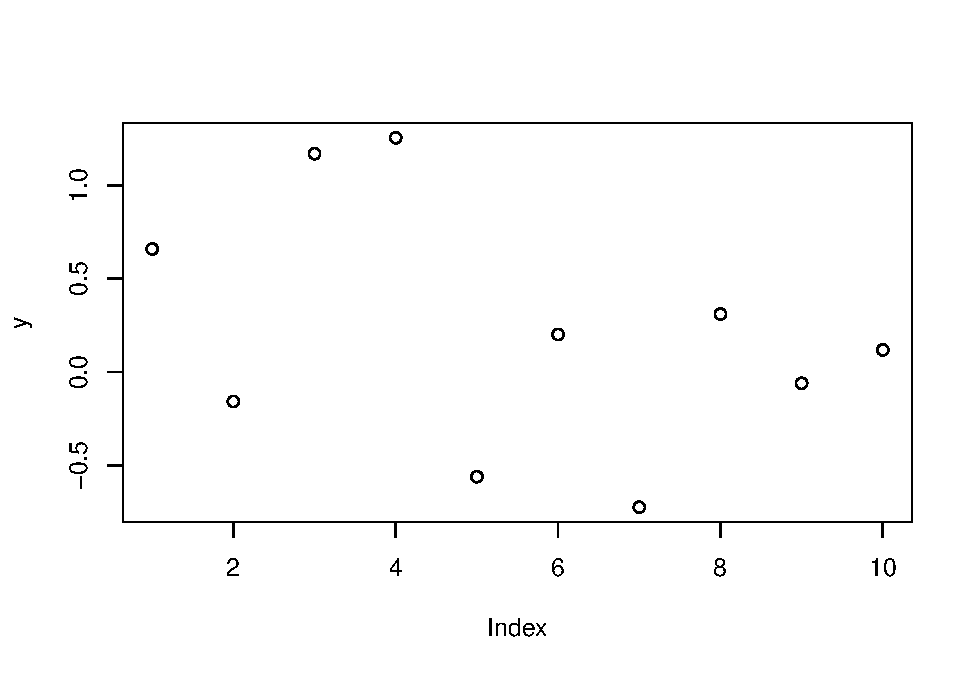
\includegraphics{_main_files/figure-latex/loaddataset-1.pdf}

\hypertarget{question-7}{%
\chapter{Question 7}\label{question-7}}

\begin{Shaded}
\begin{Highlighting}[]
\FunctionTok{summary}\NormalTok{(cars)}
\end{Highlighting}
\end{Shaded}

\begin{verbatim}
##      speed           dist       
##  Min.   : 4.0   Min.   :  2.00  
##  1st Qu.:12.0   1st Qu.: 26.00  
##  Median :15.0   Median : 36.00  
##  Mean   :15.4   Mean   : 42.98  
##  3rd Qu.:19.0   3rd Qu.: 56.00  
##  Max.   :25.0   Max.   :120.00
\end{verbatim}

\begin{theorem}
\protect\hypertarget{thm:essai}{}\label{thm:essai}This is a \texttt{theorem} environment that can contain \textbf{any}
\emph{Markdown} syntax.
\end{theorem}

\begin{proof}
Nice proof.
\end{proof}

How is Theorem \ref{thm:essai}?

\hypertarget{section:plots}{%
\chapter{Including Plots}\label{section:plots}}

You can also embed plots, for example:

\begin{figure}
\centering
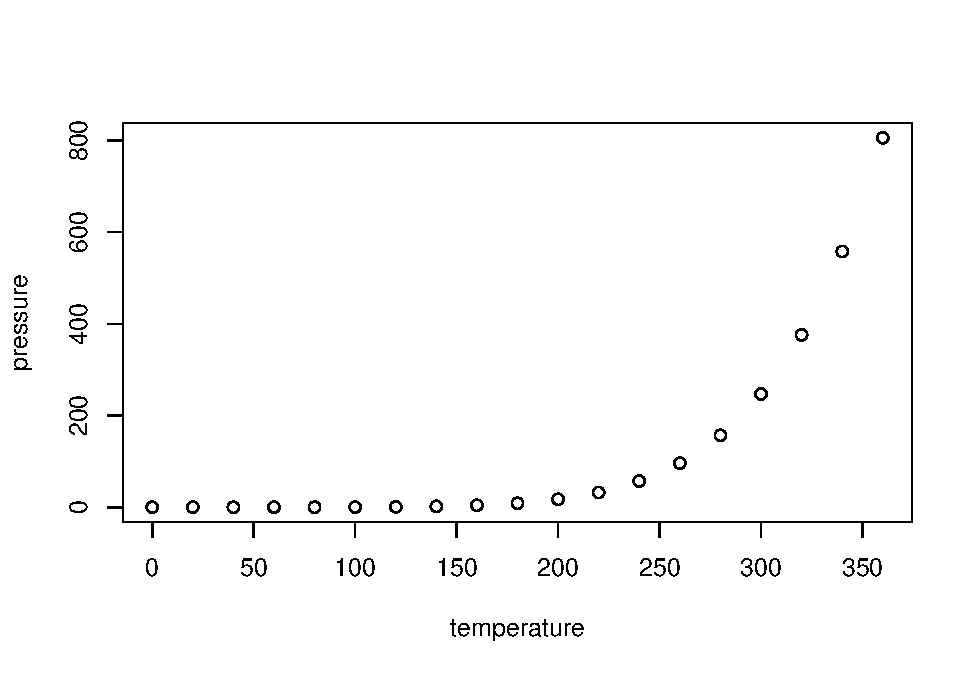
\includegraphics{_main_files/figure-latex/pressure-1.pdf}
\caption{\label{fig:pressure}This is the caption}
\end{figure}

Note that the \texttt{echo\ =\ FALSE} parameter was added to the code chunk to prevent printing of the R code that generated the plot. Figure \ref{fig:pressure} is nice!

\begin{eqnarray}
F(x) &=& 1 \\
f(y) &=& 2 \\
\int_{x=0}^\infty f(x) dx &=& 0
\end{eqnarray}

This was equation \eqref{eq:essaiRef}. See also Section \ref{section:plots}.

\begin{equation}
F(x) = 1 \label{eq:essaiRef}
\end{equation}

\begin{Shaded}
\begin{Highlighting}[]
\NormalTok{f }\OtherTok{\textless{}{-}} \ControlFlowTok{function}\NormalTok{(x)\{}\DecValTok{3}\SpecialCharTok{*}\NormalTok{x\}}
\FunctionTok{f}\NormalTok{(}\DecValTok{3}\NormalTok{)}
\end{Highlighting}
\end{Shaded}

\begin{verbatim}
## [1] 9
\end{verbatim}

\begin{itemize}
\tightlist
\item
  This is a list.
\item
  This \href{https://www.google.com}{website} is useful.
\item
  The analysis builds on \citet{dungey2009extending}
\end{itemize}

\begin{Shaded}
\begin{Highlighting}[]
\NormalTok{a }\OtherTok{\textless{}{-}} \DecValTok{3}
\FunctionTok{print}\NormalTok{(a)}
\end{Highlighting}
\end{Shaded}

\begin{verbatim}
## [1] 3
\end{verbatim}

\begin{Shaded}
\begin{Highlighting}[]
\DecValTok{2}\SpecialCharTok{*}\NormalTok{a}
\end{Highlighting}
\end{Shaded}

\begin{verbatim}
## [1] 6
\end{verbatim}

\hypertarget{question-7-1}{%
\chapter{Question 7}\label{question-7-1}}

Create some important variables for the reference person such as dummy variables for female (\(female\), 1 if female, 0 otherwise); race (\(black\), 1 if black); retired (\(retired\), 1 if labour force participation \(=\) 5); disabled (1 if labour force participation \(=\) 6); not married (\(notmar\), 1 if marital status is different from being married); full-time work (\(workft\), 1 if works full time); pat-time work (\(workpt\), 1 if works part time).

\begin{Shaded}
\begin{Highlighting}[]
\DecValTok{1}\SpecialCharTok{+}\DecValTok{1}
\end{Highlighting}
\end{Shaded}

\begin{verbatim}
## [1] 2
\end{verbatim}

\hypertarget{appendix-1}{%
\chapter{Appendix}\label{appendix-1}}

\begin{center}\rule{0.5\linewidth}{0.5pt}\end{center}

\begin{proposition}
\protect\hypertarget{prp:essai}{}\label{prp:essai}We have:
\[
f_{X|Y}(x,y)=\frac{f_{XY}(x,y)}{f_Y(y)}.
\]
\end{proposition}

\begin{center}\rule{0.5\linewidth}{0.5pt}\end{center}

\begin{proof}
We have:
\begin{eqnarray*}
f_{X|Y}(x,y)&=&\lim_{\varepsilon \rightarrow 0} \frac{\mathbb{P}(x < X \le x + \varepsilon|Y=y)}{\varepsilon}\\
&=&\lim_{\varepsilon \rightarrow 0} \frac{1}{\varepsilon}\mathbb{P}(x < X \le x + \varepsilon|y<Y\le y+\varepsilon)\\
&=&\lim_{\varepsilon \rightarrow 0} \frac{1}{\varepsilon}\frac{\mathbb{P}(x < X \le x + \varepsilon,y<Y\le y+\varepsilon)}{\mathbb{P}(y<Y\le y+\varepsilon)}\\
&=&\lim_{\varepsilon \rightarrow 0} \frac{1}{\varepsilon} \frac{\varepsilon^2f_{XY}(x,y)}{\varepsilon f_{Y}(y)}.\square
\end{eqnarray*}
\end{proof}

\hypertarget{references}{%
\chapter{References}\label{references}}

\hypertarget{methods}{%
\chapter{Methods}\label{methods}}

We describe our methods in this chapter.

Math can be added in body using usual syntax like this

\hypertarget{math-example}{%
\section{math example}\label{math-example}}

\(p\) is unknown but expected to be around 1/3. Standard error will be approximated

\[
SE = \sqrt(\frac{p(1-p)}{n}) \approx \sqrt{\frac{1/3 (1 - 1/3)} {300}} = 0.027
\]

You can also use math in footnotes like this\footnote{where we mention \(p = \frac{a}{b}\)}.

We will approximate standard error to 0.027\footnote{\(p\) is unknown but expected to be around 1/3. Standard error will be approximated

  \[
  SE = \sqrt(\frac{p(1-p)}{n}) \approx \sqrt{\frac{1/3 (1 - 1/3)} {300}} = 0.027
  \]}

\hypertarget{applications}{%
\chapter{Applications}\label{applications}}

Some \emph{significant} applications are demonstrated in this chapter.

\hypertarget{example-one}{%
\section{Example one}\label{example-one}}

\hypertarget{example-two}{%
\section{Example two}\label{example-two}}

\hypertarget{final-words}{%
\chapter{Final Words}\label{final-words}}

We have finished a nice book.

  \bibliography{book.bib,packages.bib}

\end{document}
